\chapter{System monitorowania Icinga}
\label{chap:Icinga}

W~rozdziale \ref{chap:Systemy} została przeprowadzona analiza
dostępnych na ryku systemów monitorowania. Na jej podstawie dokonano
wyboru systemu Icinga jako podstawy do budowy systemu uwzględniającego
wymagania dotyczące klienta mobilnego. System monitorujący jest bytem
złożonym. Można w~nim wyróżnić część podstawową, która stanowi
szkielet i~pozwala na funkcjonowanie głównych mechanizmów. Ponadto,
w~celu umożliwienia dostosowania systemu do indywidualnych potrzeb,
opracowany został szereg dodatków, czyli narzędzi pozwalających na
rozszerzanie funkcjonalności systemu. Mnogość dostępnych elementów
przekłada się również na duży zbiór dostępnych konfiguracji. Rozdział
ten zawiera opis podstawowych elementów systemu Icinga oraz wybranego
podzbioru dodatków, które są istotne w~kontekście tej pracy. Zawarto
tutaj również opis kilku wybranych konfiguracji, które potwierdzają
elastyczność wybranego systemu monitorowania.

\section[Opis systemu][Opis systemu]{Opis systemu}


Podstawowym elementem systemu monitorowania Icinga jest rdzeń
monitorujący. Jego architektura została przedstawiona na
rys. \ref{fig:icingaCoreArch}. Jest to centralne miejsce w~którym
wykonuje się przetwarzanie danych o~urządzeniach i~usługach. Dane,
które mają być przetworzone mogą zostać dostarczone na dwa sposoby.

\begin{figure}[ht]
  \caption{Schemat architektury rdzenia monitorującego systemu
    Icinga.}
  \label{fig:icingaCoreArch}
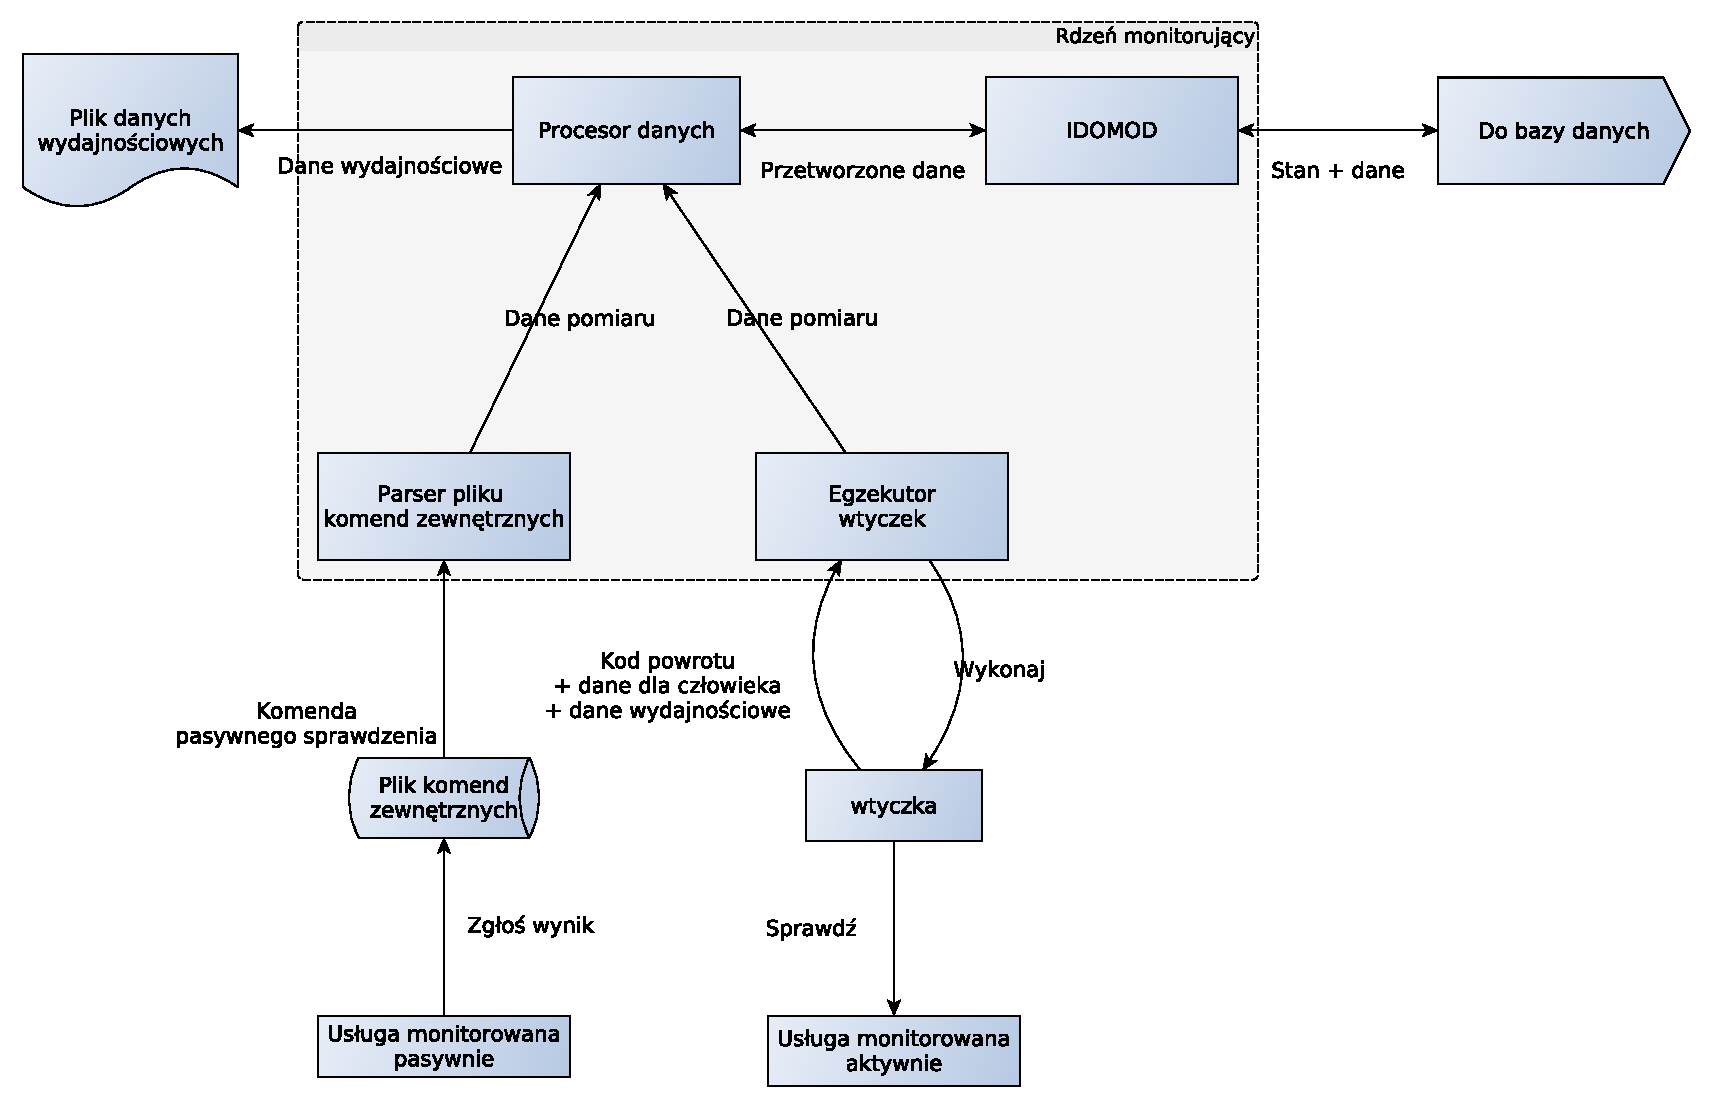
\includegraphics[width=1\textwidth]{img/icingaCoreArch}
\end{figure}


Podstawowy sposób dostarczania danych do przetworzenia opiera się na
monitorowaniu aktywnym. W~systemie Icinga monitorowanie aktywne odbywa
się poprzez uruchamianie w~określonych odstępach czasowych komend
zdefiniowanych przez użytkownika w~pliku konfiguracyjnym. Standardowa
komenda sprowadza się do uruchomienia wybranego przez administratora
programu z~odpowiednimi parametrami. W~ramach wykonania komendy
uruchomiony może zostać dowolny program lub skrypt. Aby jednak
zapewnić poprawne funkcjonowanie całego systemu, niezbędne jest
napisanie programu w~zgodności z~regułami opisanymi
w~\cite{www:NagiosPluginsTutorial}. Reguły te definiują jakie dane
i~w~jaki sposób powinny być przekazane z~programu (wtyczki) do rdzenia
systemu monitorującego. Pierwszym elementem przekazu danych jest
zwrócenie przez wtyczkę odpowiedniego kodu zakończenia
programu. Poszczególne wartości zwrócone mają następujące znaczenie
dla rdzenia monitorującego:

\begin{description}
\item[0] OK, wtyczka mogła wykonać sprawdzenie i~usługa lub urządzenie
  jest w~stanie OK
\item[1] WARNING, wtyczka mogła wykonać sprawdzenie ale parametry
  urządzenia lub usługi przekraczają poziom ostrzegawczy.
\item[2] CRITICAL, wtyczka mogła wykonać sprawdzenia ale parametry
  urządzenia lub usługi przekraczają poziom krytyczny.
\item[3] UNKNOWN, wtyczka nie była w~stanie wykonać sprawdzenia ze
  względu na dostarczenie nie prawidłowych parametrów wywołania lub
  niskopoziomowego błędu systemu.
\end{description}

Każda wtyczka poza numerycznym kodem wyjścia z~programu, może
przekazać do rdzenia monitorującego dane w postaci tekstowej. Dane te
powinny być wypisane na standardowe wyjście wtyczki. Składają się one
z~dwóch części. Część przed znakiem~| stanowi czytelny dla człowieka
opis stanu parametru badanego przez wtyczkę. Część znajdująca się po
tym znaku to tak zwane dane wydajnościowe. Powinny być one przekazane
w~formacie klucz=wartość gdyż są przeznaczona do dalszej obróbki przez
program.

Drugą dostępną metodą dostarczenia danych w~celu przetworzenia ich
przez rdzeń monitorujący jest plik komend zewnętrznych. Pozwala on na
monitorowanie usług w~sposób pasywny. Nie jest to tak właściwie plik
lecz potok nazwany. W~rdzeniu monitorującym obecny jest element, który
odpowiedzialny jest za czytanie danych z~potoku. Do potoku mogą być
zapisywane dowolne spośród komend przedstawionych
w~\cite[412-436]{www:IcingaDoc}. Rdzeń monitorujący po przeczytaniu
każdej komendy wykona akcję z~nią powiązaną. Szczególnym przypadkiem
komendy jest żądanie przetworzenia pasywnego sprawdzenia danej usługi
lub urządzenia. Dokładny format tej komendy został opisany
w~\cite[296-299]{www:IcingaDoc}. Należy zwrócić uwagę na dodatkowe w
stosunku do sprawdzenia aktywnego pola. Pierwsze z pól to stempel
czasu, kiedy zostało wykonane dane sprawdzenie. Kolejne dwie dodatkowe
wartości czyli nazwa urządzenia oraz usługi konieczne są w~celu
poprawnej identyfikacji usługi, której dotyczą przekazywane
dane. Reszta komendy zawiera dane o~znaczeniu znanym z~monitorowania
aktywnego.

Wykonanie zapisu do potoku nazwanego należącego do procesu rdzenia
monitorującego wymaga, aby program, który chce to zrobić uruchomiony
był na tym samym systemie co rdzeń. Aby umożliwić przekazywanie tych
danych z~innego urządzenia opracowany został program NSCA
dystrybuowany jako dodatek do systemów Nagios oraz Icinga. Specyfikuje
on protokół komunikacyjny, który pozwala na przekazanie z~innego
systemu do rdzenia monitorującego wiadomości zawierającej wynik
sprawdzenia. Program ten został szeroko opisany w~\ref{sec:NSCA}.


Otrzymane dane są w~kolejnym etapie przetwarzane przez rdzeń
sprawdzający niezależnie od sposobu ich dostarczenia. Pierwszym etapem
przetwarzania tych danych jest wydzielenie z~nich danych
przeznaczonych dla człowieka oraz danych wydajnościowych
przeznaczonych do przetwarzania przez inne dodatki. Dane wydajnościowe
zawierają wyniki pomiarów przeprowadzonych przez wtyczkę w~trakcie
determinowania jej stanu. Po wydzieleniu zostają one udostępnione na
zewnątrz rdzenia monitorującego poprzez pliki tekstowe o~zadanym w
konfiguracji formacie. Dane te są wykorzystywane przez dodatki
przeznaczone do generacji wykresów takie jak opisany w
\ref{sec:inGraph} dodatek inGraph. Poza eksportem danych
wydajnościowych w~ramach przetwarzania dokonywane jest wyznaczenie
stanu usługi na podstawie danych poprzednich oraz nowo
dostarczonych. W~minimalnej i~rzadko stosowanej konfiguracji na
podstawie przetworzonych danych, a także wszystkich danych odczytu
(również wydajnosciowych) uaktualniane są pliki przechowujące aktualne
stany usług. W~typowej konfiguracji używa się jednak komponentu
IDOUtils, który pozwala na przechowywanie stanu oraz konfiguracji
w~relacyjnej bazie danych. Dodatek ten został szczegółowo opisany
w~\ref{sec:IDOUtils}.

Interakcja systemu Icinga z użytkownikiem odbywa się poprzez interfejs
graficzny będący stroną internetową. Oczywistym jest, że do jej
prawidłowego funkcjonowania konieczny jest serwer http
np. Apache. System Icinga udostępnia dwa interfejsy
użytkownika. Pierwszym z nich jest interfejs klasyczny wykonany
w~technologi CGI, odziedziczony po systemie Nagios. Dane wyświetlane
przez ten interfejs pochodzą z~plików stanu rdzenia
monitorującego. Wszelkie informacje o~akcjach zleconych przez
administratora są natomiast przekazywane poprzez plik komend
zewnętrznych. Powyższe metody komunikacji determinują, iż interfejs
klasyczny musi znajdować się na tym samym urządzeniu co rdzeń
monitorujący. Zupełnie inny model komunikacji jest wykorzystywany
przez drugi interfejs --- icinga-web. Jest to nowoczesny serwis
internetowy zaimplementowany w~języku PHP. Do jego poprawnego
funkcjonowania konieczne jest, aby rdzeń monitorujący korzystał
z~dodatku IDOUtils. Obustronna komunikacja odbywa się wówczas poprzez
bazę danych. Umożliwia to umieszczenie rdzenia, bazy danych oraz
interfejsu użytkownika na zupełnie innych maszynach. Warto w~tym
miejscu zaznaczyć, że interfejs icinga-web wykorzystuje tak na prawdę
dwie bazy danych. Pierwsza z~nich jest wykorzystywana do komunikacji
z~rdzeniem monitorującym, natomiast druga służy do przechowywania
konfiguracji samego interfejsu graficznego.


\section[Komponent IDOUtils][Komponent IDOUtils]{Komponent IDOUtils}
\label{sec:IDOUtils}

Komponent IDOUtils jest to zestaw programów, dzięki którym możliwe jest
składowanie informacji generowanych przez rdzeń monitorujący w~bazie
danych. W~wersji dostępnej podczas pisania tej pracy wspierane były
następujące systemy zarządzania bazą danych:

\begin{itemize}
\item MySql,
\item PostgreSQL,
\item Oracle.
\end{itemize}

W~celu zapewnienia funkcjonalności omawianego komponentu, konieczne
jest utworzenie bazy danych o~odpowiednim schemacie, który został
opisany w~\cite[669-750]{www:IcingaDoc}. Udostępnione zostały również
skrypty SQL, które definiują odpowiednie tabele. Ponadto administrator
musi zapewnić odpowiednią konfigurację bazy danych, w~tym konto
użytkownika i~hasło, w~taki sposób, aby umożliwić odpowiednim
elementom komponentu IDOUtils dostęp do bazy danych.

W~celu odciążenia urządzenia, na którym uruchomiony jest system
Icinga. Komponent ten został podzielony na kilka elementów, które
mogą znajdować się na różnych urządzeniach. Można wyróżnić następujące
elementy:

\begin{description}
\item[IDOMOD] moduł rdzenia monitorującego, który pozwala mu na dostęp
  do bazy danych
\item[LOG2IDO] program pozwalający na import utworzonych wcześniej
  plików do bazy danych
\item[FILE2SOCK] program pozwalający na przekierowanie danych
  zapisywanych do pliku do gniazda TCP lub Unix
\item[IDO2DB] demon, który jest odpowiedzialny za wykonywanie operacji
  na bazie danych
\end{description}

\begin{figure}[ht]
  \caption{Schemat integracji IDOUtils z systemem Icinga.}
  \label{fig:IDOUtilsArch}
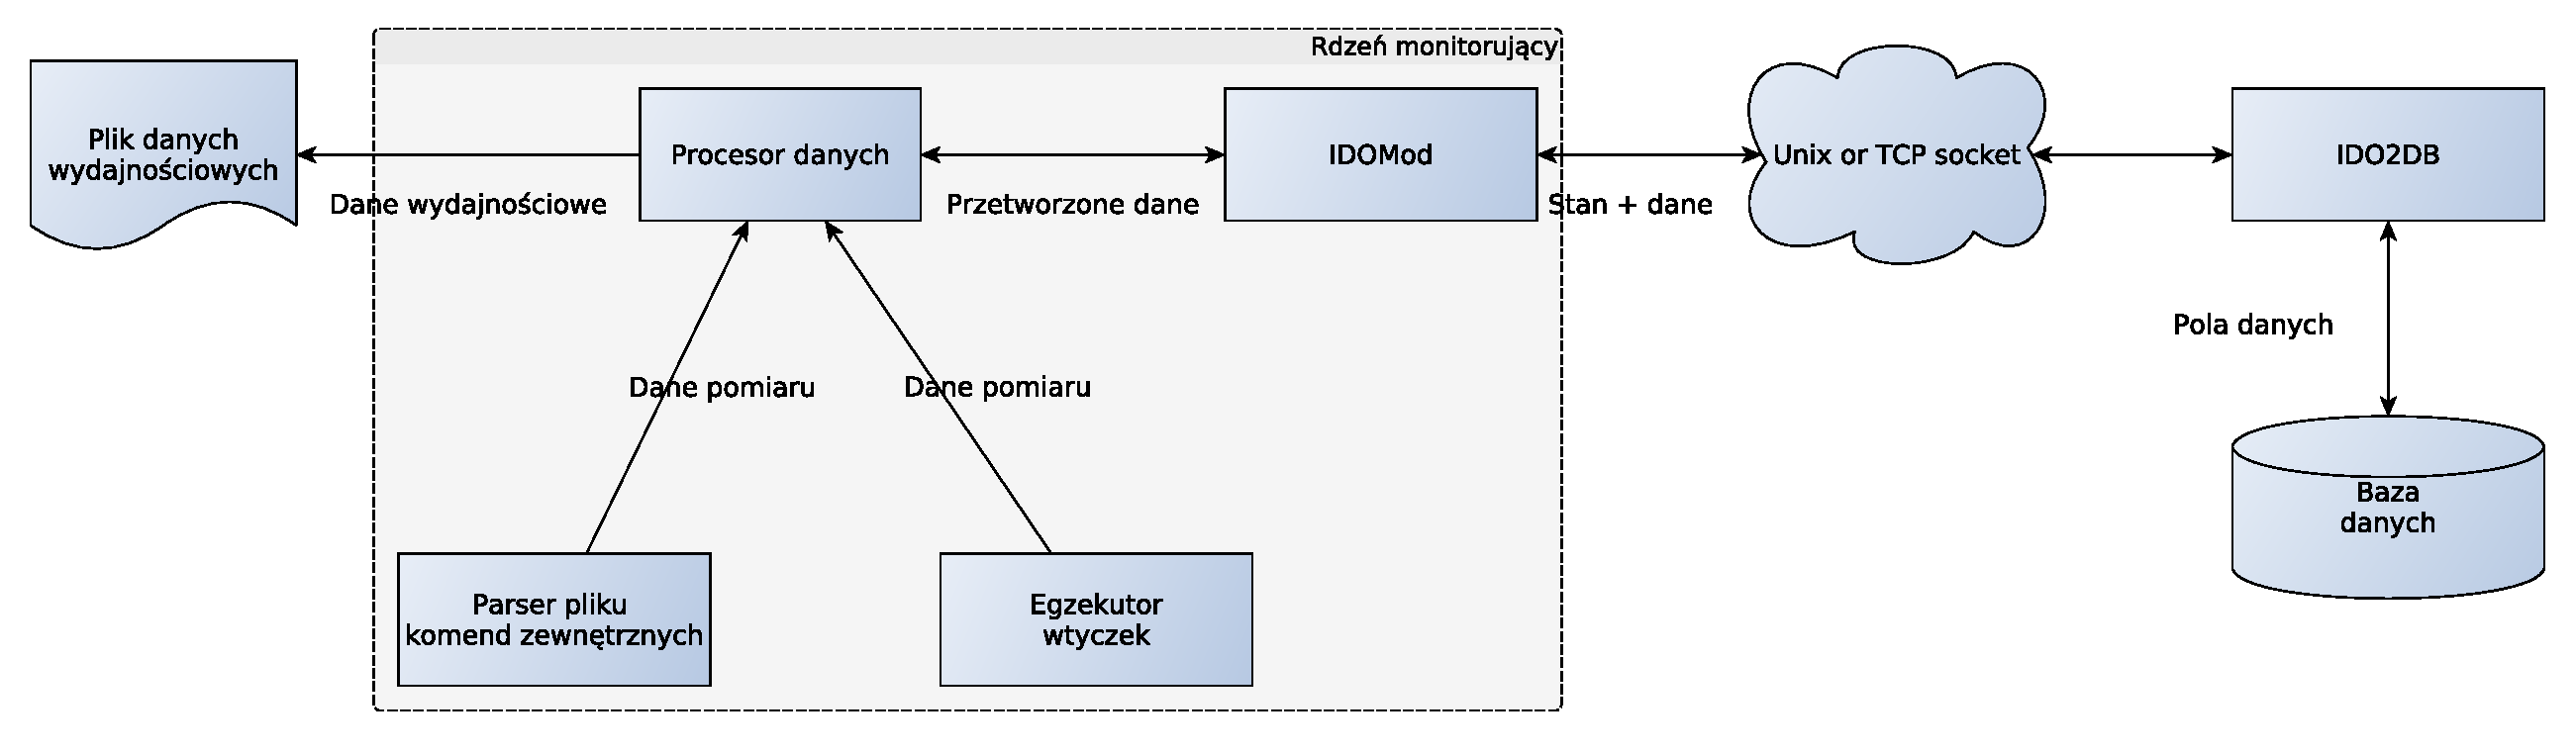
\includegraphics[width=1\textwidth]{img/idoutilsArch}
\end{figure}

Podstawowymi elementami całego komponentu są IDOMOD oraz
IDO2DB. Schemat ich typowego zastosowania przedstawiono na
rys.~\ref{fig:IDOUtilsArch}. Moduł rdzenia IDOMOD ładowany jest przez
rdzeń systemu Icinga tuż po starcie. Po załadowaniu zapewnia on spójny
interfejs do uzyskiwania danych dla wszystkich pozostałych części
rdzenia monitorującego. Ponieważ wykonywanie operacji na bazie danych
może być czasochłonne nie powinno być to wykonywane przez rdzeń
monitorujący. Z~tego powodu powstał program IDO2DB. Jest on
uruchomiony jako demon na dowolnym urządzeniu. Zadaniem tego serwisu
jest fizyczna realizacja żądań na bazie danych. Na schemacie celowo
pominięto pozostałe elementy tego komponentu, gdyż stanowią one
jedynie inne źródło danych dla demona IDO2DB i~są konieczne jedynie
przy imporcie danych historycznych z~starej instalacji systemu, lub
bardziej zaawansowanych konfiguracjach.

Ponieważ rdzeń monitorujący oraz demon IDO2DB mogą znajdować się
zarówno na jednym urządzeniu jak i~na różnych urządzeniach konieczne
jest zapewnienie odpowiednich mechanizmów komunikacji pomiędzy nimi.
Gdy programy te znajdują się na różnych urządzeniach, jako mechanizm
komunikacji wykorzystywane są gniazda TCP. W~podstawowej konfiguracji
dane przekazywane są w~sposób niezaszyfrowany. Jeśli jednak istnieje
potrzeba zapewnienia tajności oraz integralności przekazywanych danych
możliwe jest użycie protokołu SSL\footnote{ ang. {\em Secure Socket
    Layer} -- protokół warstwy prezentacji, zapewniający poufność oraz
  integralność przesyłanych danych.}. W~sytuacji gdy oba programy
uruchomione są na tym samym urządzeniu, w~celu poprawy wydajności
możliwe jest użycie gniazd protokołu Unix\footnote{ and. {\em Unix
    Domain Socket} -- metoda komunikacji między procesowej w~systemach
  Unix. Posiada jednolite API jak gniazda domeny
  internetowej.}. Najpopularniejszy sposób użycia został przedstawiony
schematycznie na~rys.~\ref{fig:IDOUtils}.

\begin{figure}[ht]
  \caption{Schemat wykorzystania IDOUtils w systemie Icinga.}
  \label{fig:IDOUtils}
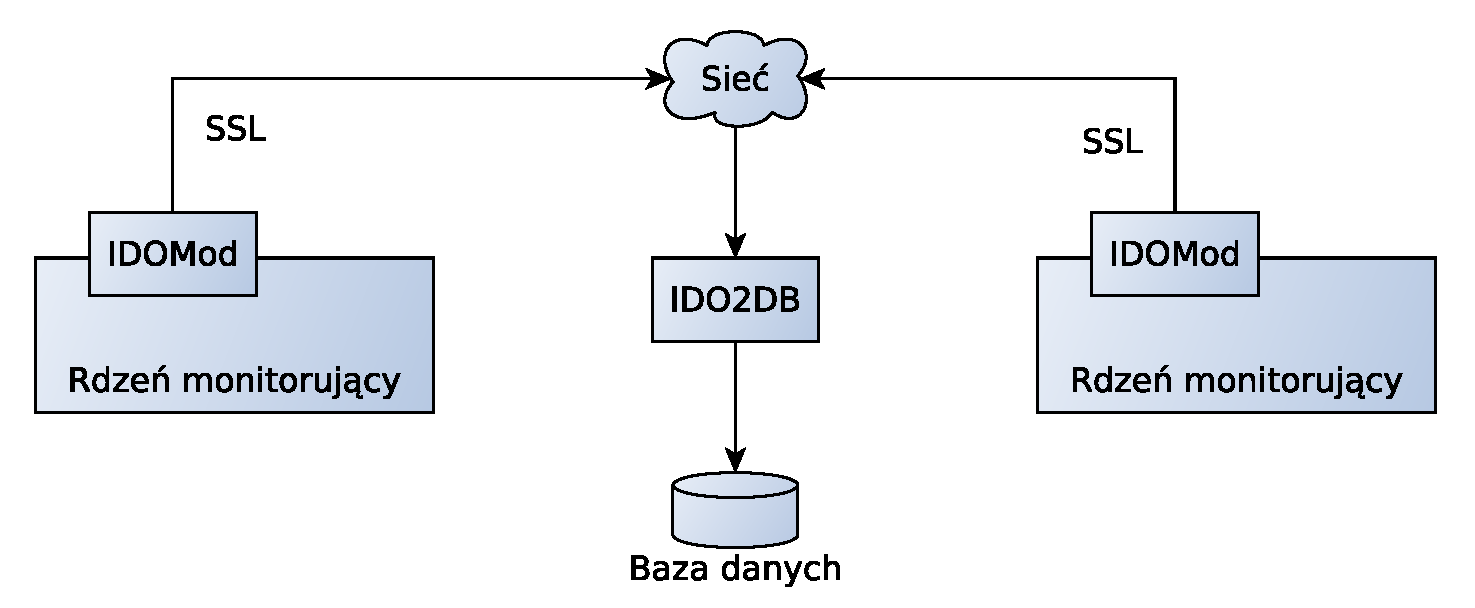
\includegraphics[width=1\textwidth]{img/idoutils}
\end{figure}

W~celu zapewnienia możliwości migracji z~środowiska, które korzystało
wcześniej z~przechowywania danych w~plikach, został dostarczony
program LOG2IDO. Pozwala on, na import danych historycznych do bazy
danych. Program ten, analogicznie jak IDOMOD nie operuje bezpośrednio
na bazie danych, lecz komunikuje się tymi samymi metodami co IDOMOD
z~demonem IDO2DB. Zarówno program LOG2IDO jak i~moduł IDOMOD mogą
kierować żądania do IDO2DB poprzez plik. W~celu zapewnienia
przekazywania tych danych z~pliku do demona IDO2DB opracowano program
FILE2SOCK. Jest to prosty program, który przekazuje dane zapisane do
danego pliku do demona IDO2DB. Program ten nie zajmuje się w~żadnym
stopniu przetwarzaniem odczytaniem danych, lecz jedynie przesłaniem ich
poprzez gniazdo internetowe lub Unix do demona IDO2DB.

\section[Dodatek inGraph][Dodatek inGraph]{Dodatek inGraph}
\label{sec:inGraph}

inGraph jest dodatekiem do systemów Icinga oraz Nagios, który
umożliwia prezentację danych zgromadzonych poprzez system monitorujący
w~postaci wykresów. Dodatek ten został opracowany przez firmę NETWAYS
GmbH i~wydany na licencji GPL w~wersji 3. Cechą, która odróżnia
dodatek inGraph od innych rozwiązań, przeznaczonych do analizy danych
historycznych jest wykorzystanie relacyjnej bazy danych do
przechowywania danych otrzymanych od systemu monitorującego. Na
podstawie otrzymanych danych dodatek inGraph dokonuje przeliczeń dla
odpowiednich przedziałów czasowych, które używane są do późniejszej
generacji wykresów. Rozmiary przedziałów definiowane są przez
użytkownika w plikach konfiguracyjnych. Wykorzystanie tego rodzaju
bazy danych powoduje nieustanny wzrost rozmiaru bazy. W celu
optymalizacji zajętości przestrzeni dyskowej dodatek inGraph
administruje danymi zgodnie z polityką zdefiniowaną w plikach
konfiguracyjnych. Dla każdego przedziału czasowego zdefiniowany jest
również okres przechowywania danych. Dodatek umożliwia przeglądanie
danych dokładnych z najmniejszych przedziałów czasu, jak i~wykresów
długoterminowych prezentujących trendy danej wartości. Ponieważ dane
są bezpośrednio administrowane przez dodatek inGraph, możliwa jest
zmiana czasów przechowywania danych z wskazanych przedziałów nawet w
trakcie działania systemu\footnote{Dla porównania należy przypomnieć
  systemy oparte na cyklicznych baza danych, gdzie rozmiar definiowany
  może być tylko i wyłącznie podczas tworzenia bazy.}.

Dodatek inGraph składa się z~dwóch niezależnych elementów,
komunikujących się poprzez XML-RPC\footnote{ang. {\em XML Remote
    Procedure Call} -- zdalne wywołanie procedur przy użyciu
  XML. Metoda zdalnego wywoływania funkcji oparta na dokumentach w
  formacie XML. Szczegółowy opis w~\cite{www:XMLRPC}.}:

\begin{itemize}
\item interfejs graficzny,
\item rdzeń zbierający dane.
\end{itemize}

\begin{figure}[ht]
  \caption{Typowy przepływ danych przy wykorzystaniu dodatku inGraph.}
  \label{fig:inGraphFlow}
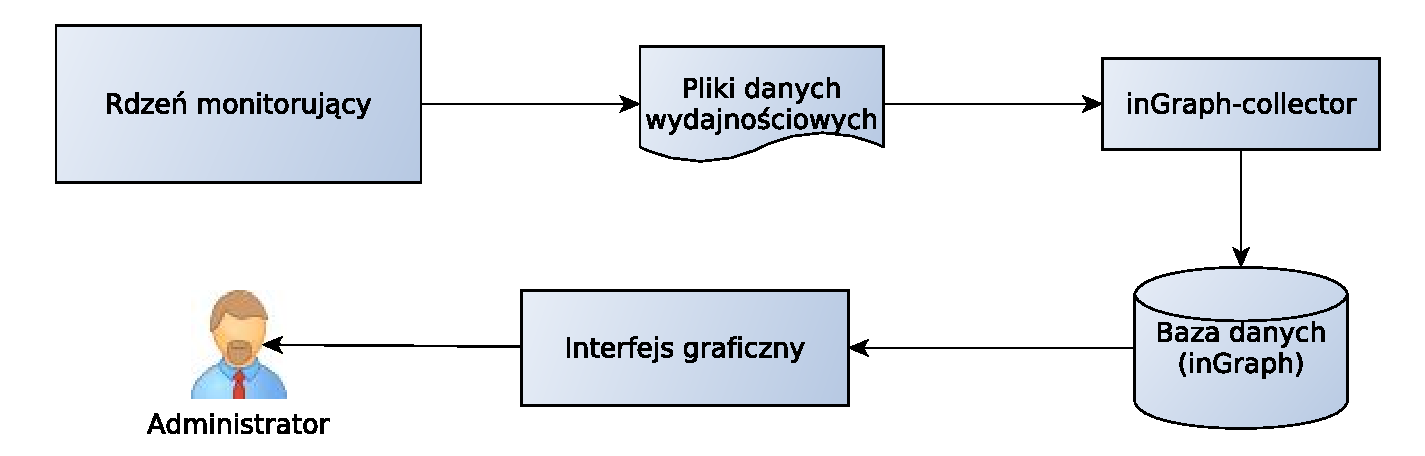
\includegraphics[width=1\textwidth]{img/ingraphFlow}
\end{figure}

Rdzeń zbierający oraz przetwarzający dane został napisany w~języku
Pythoni nosi nazwę ingraph-collector. Jego zadaniem jest pobieranie
danych od systemu monitorującego, dokonywanie ich przeliczeń, oraz
umieszczanie ich wyników w~bazie danych. Do pobierania danych
z~systemu monitorującego wykorzystano mechanizm udostępniania danych
wydajnościowych. System monitorujący musi eksportować dane przy pomocy
formatu zrozumiałego dla dodatku inGraph. Demon ingraph-collector
wykonuje ich analizę, a~następnie wykonuje wszystkie niezbędne
obliczenia np średnich wartości w~zadanych przedziałach czasowyc.,
Wyniki zapisywane są w~bazie danych MySQL lub PostgreSQL programu
inGraph. Należy zwrócić uwagę iż jest to inna baza danych, niż ta z
której korzysta system Icinga. Ważną różnicą pomiędzy danymi
składowanymi w~tej bazie, a~danymi przechowywanymi przez system
monitorujący jest ich format. Systemy monitorujące przechowują
w~postaci numerycznej jedynie skwantowany stan danej usługi lub
urządzenia (OK, WARNING itd), pozostałe dane przechowywane są
w~postaci tekstowej w~formie przekazanej przez wtyczkę. Dodatek
inGraph przechowuje natomiast w~swojej bazie dane w~postaci już
przetworzonej. Oznacza to, iż dokonywany jest rozbiór składniowy
rezultatów pomiarów i~w~bazie danych zapamiętywane są pochodzące
z~tych rezultatów dane w~postaci numerycznej. Typowy przepływ danych
został przedstawiony na~\ref{fig:inGraphFlow}.

Interfejs użytkownika dodatku inGraph został napisany w~językach PHP
oraz JavaScript. Umożliwia on podgląd danych zebranych
i~przetworzonych przez rdzeń dodatku. Interfejs może funkcjonować
zarówno jako niezależny serwis jak i~jako integralna część interfejsu
systemu Icinga. Umożliwia on generację wykresów dla każdego z~urządzeń
oraz dla każdej z usług. Formaty wykresów, a~także przedziały
agregacji danych, definiowane są w~plikach konfiguracyjnych w formacie
JSON\footnote{ang. {\em JavaScrip Object Notation} -- lekki format
  tekstowy wymiany danych komputerowych. Szczegółowo opisany
  w~\cite{www:JSON}.}.  Użytkownik po wybraniu usługi lub urządzenia
uzyskuje interaktywny wykres przezentujący dane w~zadanym
okresie. Wszystkie wykresy wygenerowane przez program są w~pełni
konfigurowalne jak i~edytowalne. Typ prezentowanych danych jest
uzależniony od rozmiaru przedziału czasu, w~którym generowany jest
wykres. 

\begin{figure}[ht]
  \caption{Interfejs dodatku inGraph.}
  \label{fig:inGraph}
\includegraphics[width=1\textwidth]{img/ingraph.png}
\end{figure}

Jeśli okno czasu jest odpowiednio małe, na wykresie zostaną
przedstawione dane dokładne. W~sytuacji, gdy nie jest możliwe
przedstawienie danych dokładnych, ze względu na rozmiar zadanego
okresu czasu, dane są agregowane w~przedziały, a~na wykresie
udostępniana jest wartość minimalna, maksymalna oraz średnia dla
danego przedziału agregacji danych. Przykładowe wykresy wygenerowane
przy pomocy dodatku inGraph przedstawia
rys. \ref{fig:inGraph}. Szczególną uwagę warto zwrócić na szare pola
reprezentujące minimum oraz maksimum w~danym przedziale.


\section[Dodatek NSCA][Dodatek NSCA]{Dodatek NSCA}
\label{sec:NSCA}

NSCA - Nagios Service Check Acceptor jest to dodatek do systemów
monitorujących z rodziny Nagios, więc również systemu Icinga. Pozwala
on na wykorzystanie mechanizmów pasywnego monitorowania z~systemu
innego niż ten, na którym uruchomione jest oprogramowanie
monitorujące. Program ten został napisany w~całości w~języku~C
i~wydany na licencji pozwalającej na wgląd do kodu
źródłowego. Wykorzystuje on plik zewnętrznych komend i~nie integruje
się z~rdzeniem monitorującym. Dzięki temu możliwe jest jego
wykorzystanie go w wielu konfiguracjach bez konieczności ingerencji
w~system monitorujacy.

\subsection[Opis dodatku NSCA][Opis dodatku NSCA]{Opis dodatku NSCA}

Dodatek NSCA definiuje protokół przekazywania danych ze zdalnej
lokalizacji, do systemu, na którym uruchomiony jest rdzeń
sprawdzający. Schemat działania systemu wykorzystującego dodatek NSCA
został przedstawiony na rys. \ref{fig:nsca}. Implementacja dodatku składa
się z~dwóch modułów:

\begin{itemize}
\item moduł wysyłający (send\_nsca) służący do wysyłania wyników
  sprawdzeń z~monitorującego systemu do centralnego serwera, na którym
  umieszczony jest rdzeń systemu monitorującego odpowiedzialny za
  przetwarzanie wyników sprawdzeń,
\item moduł odbierający (nsca) służący do odbierania wyników sprawdzeń
  od klientów i~dostarczaniu ich do pliku komend zewnętrznych danego
  systemu monitorującego.
\end{itemize}

\begin{figure}[ht]
  \caption{Schemat działania dodatku NSCA.}
  \label{fig:nsca}
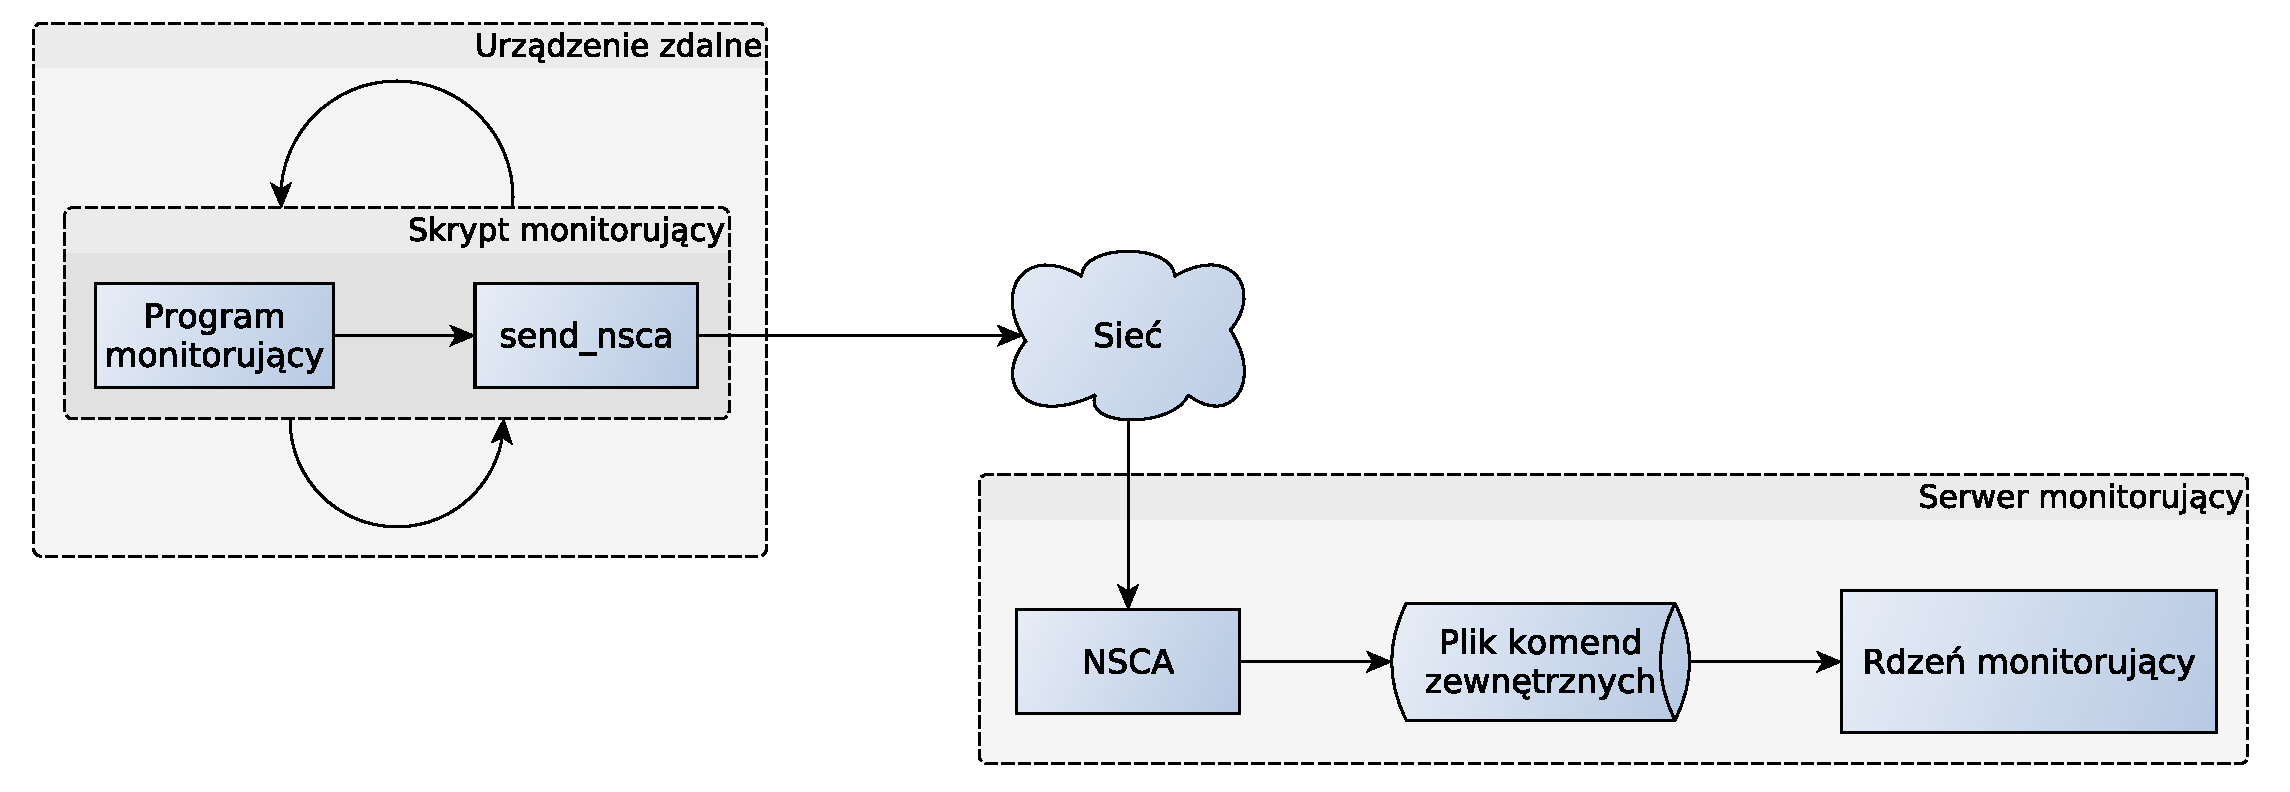
\includegraphics[width=1\textwidth]{img/nsca}
\end{figure}

%źrodło: dokumentacja w repo ?

\subsubsection[Moduł wysyłający][Moduł wysyłający]{Moduł wysyłający}
\label{subsubsec:modulWysylajacy}

Ta część dodatku uruchamiana jest na systemie, na którym funkcjonuje
jakiś mechanizm sprawdzający, który generuje wpisy dziennika. Wpisy te
po utworzeniu przekazywane są do programu wysyłającego (send\_nsca). Moduł
wysyłający, po uruchomieniu odczytuje ustawienia z~pliku
konfiguracyjnego, a~następnie próbuje połączyć się z~serwerem (NSCA). Po
udanej próbie połączenia otrzymuje pakiet inicjujący, który zawiera:

\begin{description}
\item[wektor inicjujący] wygenerowany przez serwer pseudolosowy ciąg
  znaków konieczny do inicjalizacji algorytmu kryptograficznego,
\item[stempel czasu] czas odczytany przez serwer w~chwili nadejścia
  połączenia od klienta.
\end{description} 

Po otrzymaniu pakietu inicjującego moduł wysyłający rozpoczyna
czytanie wpisów z~standardowego wejścia. Wszystkie wpisy dziennika
muszą być odpowiednio sformatowane: poszczególne pola informacyjne
muszą być rozdzielone pojedynczą tabulacją, a~cały wpis zakończony
znakiem nowej linii. Wpisy dotyczącego urządzenia powinny zawierać
następujące pola:

\begin{description}
\item[nazwa urządzenia] krótka nazwa urządzenia, którego stan jest
  przekazywany,
\item[stan] numerycznie wyrażony kod stanu urządzenia,
\item[odczyt] dodatkowe wartości odczytów opisujące stan urządzenia w~
  formacie zgodnym z formatem danych przekazywanych przez wtyczki.
\end{description}

Natomiast wpisy dotyczące usługi świadczonej przez to urządzenie, lub
innego rejestrowanego parametru tego urządzenia powinny zawierać
następujące pola:

\begin{description}
\item[nazwa urządzenia] krótka nazwa urządzenia na którym uruchomiona
  jest usługa,
\item[opis usługi] nazwa usługi danego urządzenia, której dotyczy wpis
\item[stan] numerycznie wyrażony kod stanu usługi,
\item[odczyt] dodatkowe wartości odczytów opisujące stan usługi w~
  formacie zgodnym z~formatem danych przekazywanych przez wtyczki.
\end{description}

Łatwo zauważyć, że żadne z~pól wpisu dziennika nie zawiera stempla
czasu wymaganego przez rdzeń sprawdzający przy zapamiętywaniu odczytu
pasywnego. Dzieje się tak, gdyż program NSCA posiada zdefiniowaną
własną politykę określania czasu wpisu w~dzienniku. Do każdego pakietu
zawierającego wpis dziennika dodawany jest stempel czasu otrzymany
w~pakiecie inicjującym od modułu odbierającego. Właściwy stempel
czasu, który trafia do rdzenia monitorującego nadawany jest natomiast
przez moduł odbierający.

Kolejnym krokiem działania modułu jest obliczenie cyklicznego kodu
nadmiarowego CRC32 dla danego pakietu. Po dołączeniu obliczonego kodu
do pakietu pakiet jest szyfrowany. Algorytm kryptograficzny stosowany do
szyfrowania pakietów został wcześniej zainicjalizowany wektorem
pseudolosowych danych odebranych w~pakiecie inicjalizacyjnym od modułu
odbierającego. Po zaszyfrowaniu dane są wysyłane, a~moduł wysyłający,
bez oczekiwania na potwierdzenie przetworzenia przez serwer,
rozpoczyna przetwarzanie kolejnego wpisu dziennika.

\subsubsection[Moduł odbierający][Moduł odbierający]{Moduł odbierający}

Demon, który stanowi moduł odbierający funkcjonuje na tym samym
systemie operacyjnym, na którym znajduje się rdzeń systemu
monitorującego. Ta część odpowiedzialna jest za odbieranie danych od
klientów i~przekazywanie ich do rdzenia programu monitorującego. Moduł
ten może pracować w~jednym z~poniższych trybów:

\begin{description}
\item[samodzielny demon jedno procesowy] uruchomiony w~tle demon, który
  nasłuchuje na przychodzące połączenia od klientów i~po nadejściu
  połączenia jest ono obsługiwane przy użyciu jednego procesu z~jednym
  wątkiem,
\item[samodzielny demon wieloprocesowy] uruchomiony w~tle demon,
  którego proces główny nasłuchuje na nadejście połączeń od klientów,
  gdy takie połączenie nadejdzie proces jest duplikowany i~każdy
  z~klientów obsługiwany jest w~innym procesie potomnym,
\item[demon zintegrowany z~inetd] w~systemie uruchomiony jest demon
  inetd, który nasłuchuje na połączenia od klientów na konkretnym
  gnieździe, a~gdy nadejdzie połączenie od klienta uruchamiany jest
  proces demona NSCA, który obsługuje nowe połączenie i~kończy się
  wraz z~zakończeniem obsługi klienta.
\end{description}

Do przekazywania odebranych danych używany jest mechanizm pasywnego
monitorowania dostępny w~systemach z~rodziny Nagios. Aby możliwe było
wykorzystanie tego mechanizmu do przekazania danych konieczne jest
zapewnienie demonowi NSCA dostępu do pliku zewnętrznych komend systemu
monitorującego. Ponieważ plik ten jest potokiem
nazwanym, chroniony jest on przez Uniksowy system uprawnień
użytkowników. Zapewnienie dostępu do takiego bytu może się odbyć na
dwa sposoby. Pierwszym, polecanym przez twórców systemów
monitorujących, jest uruchamianie demona NSCA jako procesu tego samego
użytkownika co proces rdzenia systemu monitorującego. Drugim sposobem
jest modyfikacja praw dostępu do omawianego pliku, tak aby umożliwić
dostęp użytkownikowi, z~którego uprawnieniami uruchomiony jest demon
NSCA. Przy zastosowaniu drugiego rozwiązania zalecana jest szczególna
ostrożność, gdyż dostęp do pliku zewnętrznych komend daje bardzo duże
możliwości ingerencji w~system monitorujący.

Komunikacja modułu odbierającego z~klientem rozpoczyna się od
nadejścia połączenia od klienta. Gdy moduł odbierający otrzyma nowe
połączenie zostanie wysłany pakiet inicjalizujący, którego zawartość
została opisana już wcześniej opisana w tym rozdziale. Po przesłaniu
pakietu inicjalizującego połączenie, moduł odbierający oczekuje na
dane od klienta. Każdy wpis dziennika przesyłany jest przy użyciu
pakietu o~poniższych polach:

\begin{description}
\item[wersja protokołu] ---  aktualnie używana wersja protokołu komunikacyjnego,
\item[kod CRC32] ---  kod CRC32 bieżącego pakietu,
\item[stempel czasu] --- stempel czasu pochodzący z~pakietu
  inicjalizującego przesłanego klientowi,
\item[kod statusu] --- kod stanu usługi/hosta powiązany z~przesyłanym wpisem
\item[nazwa hosta] --- nazwa urządzenia, które podlegał sprawdzeniu. Nie jest
  konieczne aby było to to samo urządzenie, który dostarcza dane,
\item[opis usługi] --- nazwa usługi, która podlegała sprawdzeniu lub pusty
  napis jeśli sprawdzenie dotyczy urządzenia,
\item[wynik sprawdzenia] --- napis wygenerowany przez wtyczkę, która
  dokonywała sprawdzenia, zawierający dodatkowe dane na temat stanu
  urządzenia lub usługi
\end{description}

Pakiety są zaszyfrowane z~użyciem algorytmu oraz klucza symetrycznego
pochodzącego z~pliku konfiguracyjnego demona send\_nsca. Po odebraniu
spodziewanej ilości danych (wszystkie pakiety mają taką samą długość
wynikającą z~rozmiaru struktury), następuje próba odszyfrowania
odebranych danych. Sprawdzenie poprawności odebranych danych
i~jednocześnie weryfikacja uprawnień odbywa się poprzez kontrolę
zawartości pola CRC32. Jeśli wartość znajdująca się w~tym polu zgadza
się z~wartością wyliczoną dla całości otrzymanych danych, to pakiet
jest przyjmowany, w~przeciwnym zaś razie pakiet zostanie odrzucony bez
powiadamiania o~tym jego nadawcy. Dalsze przetwarzanie otrzymanego
pakietu rozpoczyna się od porównania bieżącego stempla czasu z~tym
pochodzącym z~odebranego pakietu. Jeśli różnica pomiędzy nimi jest
zbyt duża, dane zostają odrzucone. Ostatnią czynnością wykonywaną
przez moduł odbierający jest zapisanie odebranego wpisu do pliku
zewnętrznych komend jądra systemu monitorującego.

Warto wspomnieć, że stempel czasu przesłany przez klienta nie jest
dostarczany do jądra monitorującego. Służy on jedynie określeniu
odstępu czasu od inicjalizacji sesji do chwili otrzymania wiadomości
i~podjęciu decyzji o~przyjęciu, bądź odrzuceniu pakietu. Do systemu
monitorującego trafia natomiast bieżący stempel czasu serwera, na
którym uruchomiony jest moduł odbierający i~jądro systemu
monitorującego. Do generacji stempla czasu wykorzystywany jest czas
uniwersalny. Istotną, może się również okazać informacja, iż protokół
komunikacyjny nie przewiduje przesyłania ACK\footnote {ang. {\em
    Acknowledgement} -- pozytywne potwierdzenie, powszechnie przyjęta
  nazwa komunikatu potwierdzającego przyjęcie i~przetworzenie danych
  przez aplikację}, bądź też NACK\footnote{ang. {\em Negative
    Acknowledgement} -- potwierdzenie negatywne, powszechnie przyjęta
  nazwa komunikatu oznaczająca odmowę przyjęcia lub przetworzenia
  odebranych danych}. Moduł wysyłający, ma zatem pewność, iż wysłane
przez niego dane zostaną dostarczone, gdyż używany jest protokół TCP.
Nie ma jednak żadnej gwarancji ani informacji, że dane przesłane do
modułu odbierającego zostaną dostarczone do rdzenia systemu
monitorującego.

\subsection[Bezpieczeństwo][Bezpieczeństwo]{Bezpieczeństwo}

Bezpieczeństwo monitorowania z~użyciem dodatku NSCA opiera się na
kryptografii symetrycznej oraz cyklicznym kodzie nadmiarowym
CRC32. Wiadomość inicjująca połączenie jest nieszyfrowana. Natomiast
każda wiadomość zawierająca wpisy dziennika jest zaszyfrowana
algorytmem wybranym podczas konfiguracji systemu. Dodatek NSCA
korzysta z~biblioteki libmcrypt\footnote{Szczegółowy opis biblioteki
  jak i~dostępnych w niej algorytmów można znaleźć w
  \cite{www:libmcrypt}.} i~umożliwia użycie jednego spośród wielu
algorytmów kryptografii symetrycznej, które zostały w niej
zaimplementowane. Użytkownik posiada jedynie możliwość wyboru
stosowanego algorytmu, natomiast jako tryb pracy stosowany jest tryb
sprzężenia zwrotnego szyfrogramu. Tryb ten wymaga zawsze inicjalizacji
zarówno kodera jak i~dekodera tym samym wektorem początkowym, który
w~przypadku tego protokołu, jest przesyłany przez serwer w pakiecie
inicjującym.

Wszystkie algorytmy symetryczne do prawidłowego działania wymagają,
aby komunikujące się strony współdzieliły pewien sekret jakim jest
klucz używany do szyfrowania. Ujawnienie klucza symetrycznego wiąże
się z~kompromitacją całego systemu kryptograficznego. W dodatku NSCA
klucz ten uzyskiwany jest z~hasła, które musi być zapisane przez
administratora systemu zarówno w~części odbierającej jak
i~wysyłającej. Oczywistym jest, iż poza współdzieleniem klucza,
wszystkie komunikujące się węzły muszą używać tego samego algorytmu
kryptograficznego.

Algorytmy szyfrowania zapewniają tajność przesyłanej wiadomości,
jednak w~przypadku systemu monitorowania potrzebne jest również
zapewnienie integralności. Integralność w~dodatku NSCA zapewniana jest
poprzez cykliczny kod nadmiarowy CRC32. Przed zaszyfrowaniem
wiadomości obliczany jest jej kod CRC, który jest dołączany do
wiadomości. Następnie wiadomośc jest szyfrowana i przesyłana do
serwera NSCA. Po odebraniu wiadomości jest ona odszyfrowywana
i~następuje weryfikacja kodu CRC. Jeśli weryfikacja się nie powiedzie
pakiet jest oznaczany jako dane z~naruszoną integralnością
i~w~konsekwencji odrzucany bez powiadomienia o~tym
klienta. W~szczególności, taka sytuacja może się zdarzyć, gdy klient
używa innego algorytmu kryptograficznego lub klucza. Pakiety, których
integralność nie zostanie pozytywnie zweryfikowana są odrzucane.

Model bezpieczeństwa zastosowany w~dodatku NSCA ma wiele
wad. Największą z~nich jest zastosowanie kodu CRC32 do sprawdzania
integralności przesyłanych wiadomości. Kod ten można bardzo prosto
i~szybko obliczyć, a~ponadto posiada on niewielką długość. Niestety
jest on podatny na kolizje przez co nie powinien on być stosowany do
sprawdzania integralności wiadomości. Warto przypomnieć, iż wszystkie
ustawienia zarówno modułu wysyłającego jak i~odbierającego
przechowywane są w~plikach na dyskach odpowiednich urządzeń. Pliki te
zawierają również klucze symetryczne, które są stosowane w~całym
systemie. Oznacza to, iż uzyskanie dostępu typu odczyt do takiego
pliku powoduje utratę tajności danych przesyłanych w~całym
systemie. Ponadto przyjęty model bezpieczeństwa, nie zawiera żadnej
weryfikacji danych pochodzących od klientów. Oznacza to, że każdy
klient może przesłać wpisy dziennika, udające wpisy pochodzące od
zupełnie innych klientów. W~szczególności, jeśli atakujący uzyska klucz
symetryczny, to nie tylko będzie mógł odczytywać informacje o~wpisach
przesyłanych od klientów, lecz także podszywać się pod klientów
i~przesyłać fałszywe wpisy. Taka luka może być wykorzystana przy ataku
na jakąś usługę lub urządzenie. Atakujący rozpoczyna atak, po czym
przechwytuje pakiety z~wpisami dziennika, które mogą świadczyć
o~rozpoczęciu ataku i~w~zamian przesyła do serwera fałszywe pakiety
informujące, iż wszystkie usługi pracują normalnie.

\section[Konfiguracje rozproszone][Podstawowe konfiguracje rozproszone]{Podstawowe konfiguracje rozproszone}

Podstawowa konfiguracja systemu monitorującego Icinga składa się
jedynie z~rdzenia monitorującego oraz klasycznego interfejsu
użytkownika. W~tej konfiguracji, zarówno ustawienia systemu
monitorującego, jak i~dane o~stanie usług i~urządzeń znajdują się
w~plikach lokalnych. Jeśli nie zostaną użyte żadne dodatkowe
mechanizmy transportu danych, obie części systemu Icinga będą musiały
być wykonywane na jednym urządzeniu. Jeśli monitorowana infrastruktura
jest bardzo rozbudowana, a~administrator często i~intensywnie korzysta
z~interfejsu graficznego, to umiejscowienie obu tych elementów na
jednym urządzeniu może powodować jego znaczące obciążenie i~zaburzenia
w~prawidłowym monitorowaniu infrastruktury. Należy również zwrócić
uwagę na zagadnienie bezpieczeństwa takiego rozwiązania. Jeśli
administrator chciałby udostępnić interfejs użytkownika poza
monitorowaną sieć, musi on zezwolić na dostęp z~zewnątrz do
urządzenia, które monitoruje całą infrastrukturę. Obniża to
bezpieczeństwo w~sieci, gdyż atakujący może ukierunkować swoje
działania właśnie na to urządzenie, a~uzyskanie dostępu do niego
pozwoli na ataki innych, być może słabiej zabezpieczonych urządzeń
znajdujących się w~sieci. Schemat opisanej konfiguracji przedstawiono
na \ref{fig:icingaMini}.

\begin{figure}[ht]
  \caption{Schemat minimalnej konfiguracji systemu Icinga.}
  \label{fig:icingaMini}
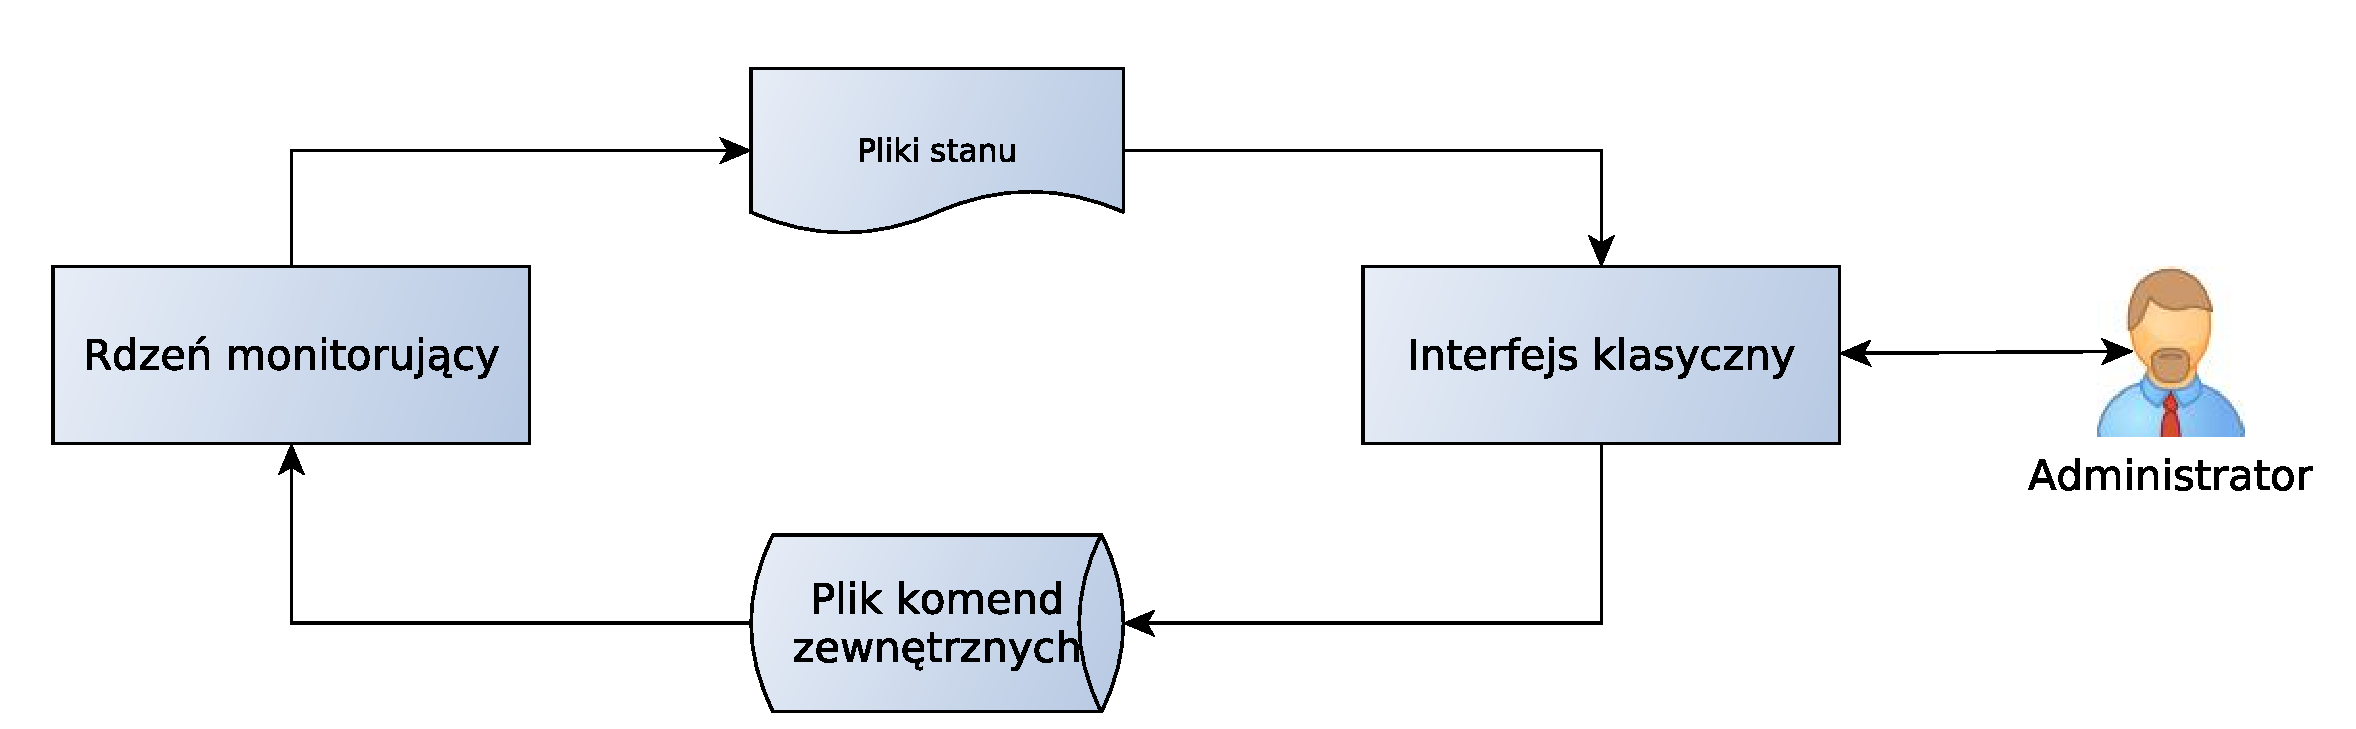
\includegraphics[width=1\textwidth]{img/icingaMini}
\end{figure}

Podstawową metodą optymalizacji przedstawionej konfiguracji jest
rozmieszczenie rdzenia monitorującego oraz interfejsu użytkownika na
różnych urządzeniach fizycznych. Umożliwienie rozdzielenia tych dwóch
bytów wymaga zapewnienia im wspólnego miejsca, w~którym składowane
będą dane konfiguracyjne, dane zawierające bieżący stan sieci oraz
reprezentację powstałych zdarzeń. System Icinga wykorzystuje do tego
celu relacyjną bazę danych. Klasyczny interfejs nie wspiera
komunikacji poprzez bazę danych, dlatego należy wykorzystać interfejs
icinga-web. Zapewnienie współpracy rdzenia monitorującego z~baza
danych odbywa się poprzez komponent IDOUtils opisany
w~rozdz.~\ref{sec:IDOUtils}. System składa się zatem z~następujących
elementów:

\begin{itemize}
\item rdzeń monitorujący wraz z~IDOMod,
\item IDO2DB
\item baza danych
\item interfejs graficzny icinga-web
\end{itemize}

Logiczny schemat konfiguracji został przedstawiony na
rys.\ref{fig:icingaBase}. Dzięki modularnej budowie całego systemu
możliwe jest umieszczenie każdego z~wymienionych elementów na osobnym
urządzaniu fizycznym.  Umożliwia to odciążenie urządzenia, na którym
uruchomiony jest rdzeń monitorujący. Ponadto zwiększone zostaje
bezpieczeństwo całego rozwiązania, gdyż konieczne jest udostępnienie
na zewnątrz jedynie serwera na którym znajduje się interfejs
sieciowy. Urządzenie to musi mieć dostęp do bazy danych, lecz nie musi
mieć dostępu do urządzenia, na którym umieszczony jest rdzeń
monitorujący oraz do całej monitorowanej infrastruktury. Pozwala to na
umieszczenie rdzenia monitorującego razem z~monitorowaną
infrastrukturą za zaporą ogniową, co ogranicza możliwości ingerencji
w~system monitorowania i~infrastrukturę sieciową.

\begin{figure}[ht]
  \caption{Schemat podstawowej konfiguracji systemu Icinga.}
  \label{fig:icingaBase}
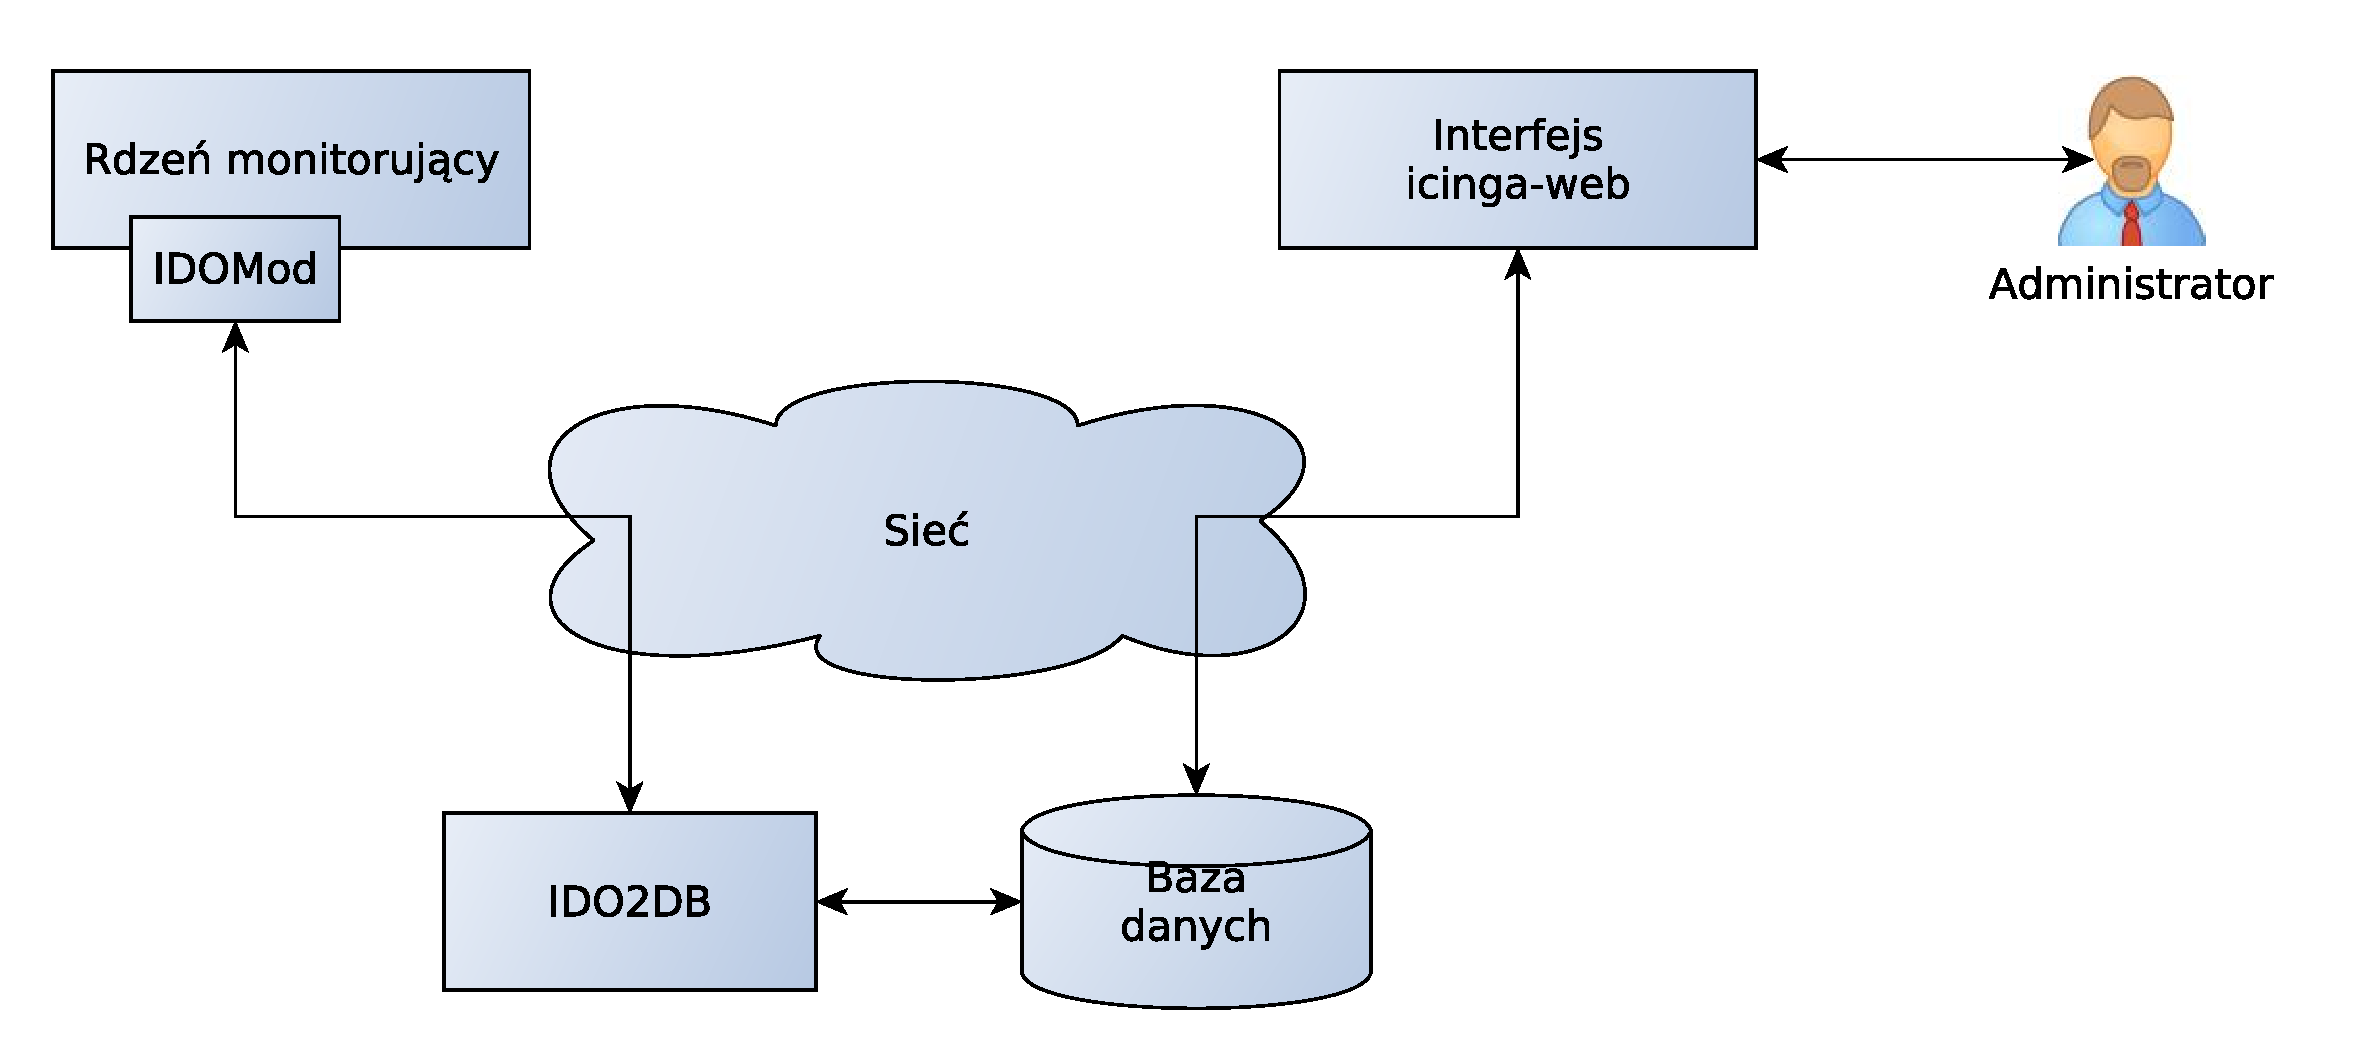
\includegraphics[width=1\textwidth]{img/icingaBase}
\end{figure}

Przedstawiona architektura stanowi bardzo dobrą konfigurację dla firm
posiadających jednolitą infrastrukturę sieciową o~średniej
wielkości. Istnieją jednak sieci dla których przedstawiona
architektura może okazać się niewystarczająca. Jedna z~takich sytuacji
ma miejsce, gdy instytucja posiada sieć złożoną z~kilku segmentów czy
to ze względu na separacje czy też lokalizacje
geograficzną. Przedstawiona architektura nie umożliwia monitorowania
aktywnego, urządzeń znajdujących się za zaporą ogniową. Możliwe jest
monitorowanie pasywne takich usług jednak wymaga ono ingerencji
w~monitorowane serwery. Kolejna z~sytuacji ma miejsce, gdy
monitorowana infrastruktura, jest na tyle rozbudowana, że urządzenie
na którym uruchomiony jest rdzeń nie posiada wystarczającej ilości
zasobów, aby monitorować wszystkie urządzenia i~usługi. Obie te
sytuacje wymagają monitorowania przy jednoczesnym użyciu wielu
instancji rdzenia monitorującego.


Pierwszy z~możliwych scenariuszy współpracy wielu instancji rdzenia
monitorującego wymaga zastosowania dodatku NSCA omówionego
w~\ref{sec:NSCA}. Konfiguracja ta zakłada istnienie jednej wyróżnionej
instancji rdzenia monitorującego, która będzie odpowiedzialna za
przetwarzanie wszystkich wyników sprawdzeń, a~także generacje zdarzeń
i~powiadomień. Konieczne jest również zapewnienie możliwości
komunikacji z~co najmniej jednego urządzenia w~każdym segmencie
sieci. Konfiguracja ta została oparta o~mechanizm pasywnego sprawdzana
usług i~urządzeń. Instancja centralna posiada wszystkie usługi
skonfigurowane w~taki sposób, aby możliwe było dostarczanie pasywnych
wyników sprawdzeń tych usług. Na tym samym systemie, co wyróżniona
instancja rdzenia uruchomiony jest również serwis systemowy NSCA,
który oczekuje na dane przesyłany z~instancji roboczych. Każda
z~instancji roboczych może zarówno wykonywać monitorowanie aktywne jak
i~pasywne pewnej części usług lub urządzeń. Wyniki sprawdzeń nie są
jednak przetwarzane przez instancję roboczą, lecz są przesyłane
z~użyciem send\_nsca do instancji centralnej, w~której następuje
odpowiednie przetwarzanie. Schemat współpracy poszczególnych elementów
systemu w tej konfiguracji zawarto na \ref{fig:rozpNSCA}.

\begin{figure}[ht]
  \caption{Schemat konfiguracji rozproszonej z~instancją centralną.}
  \label{fig:rozpNSCA}
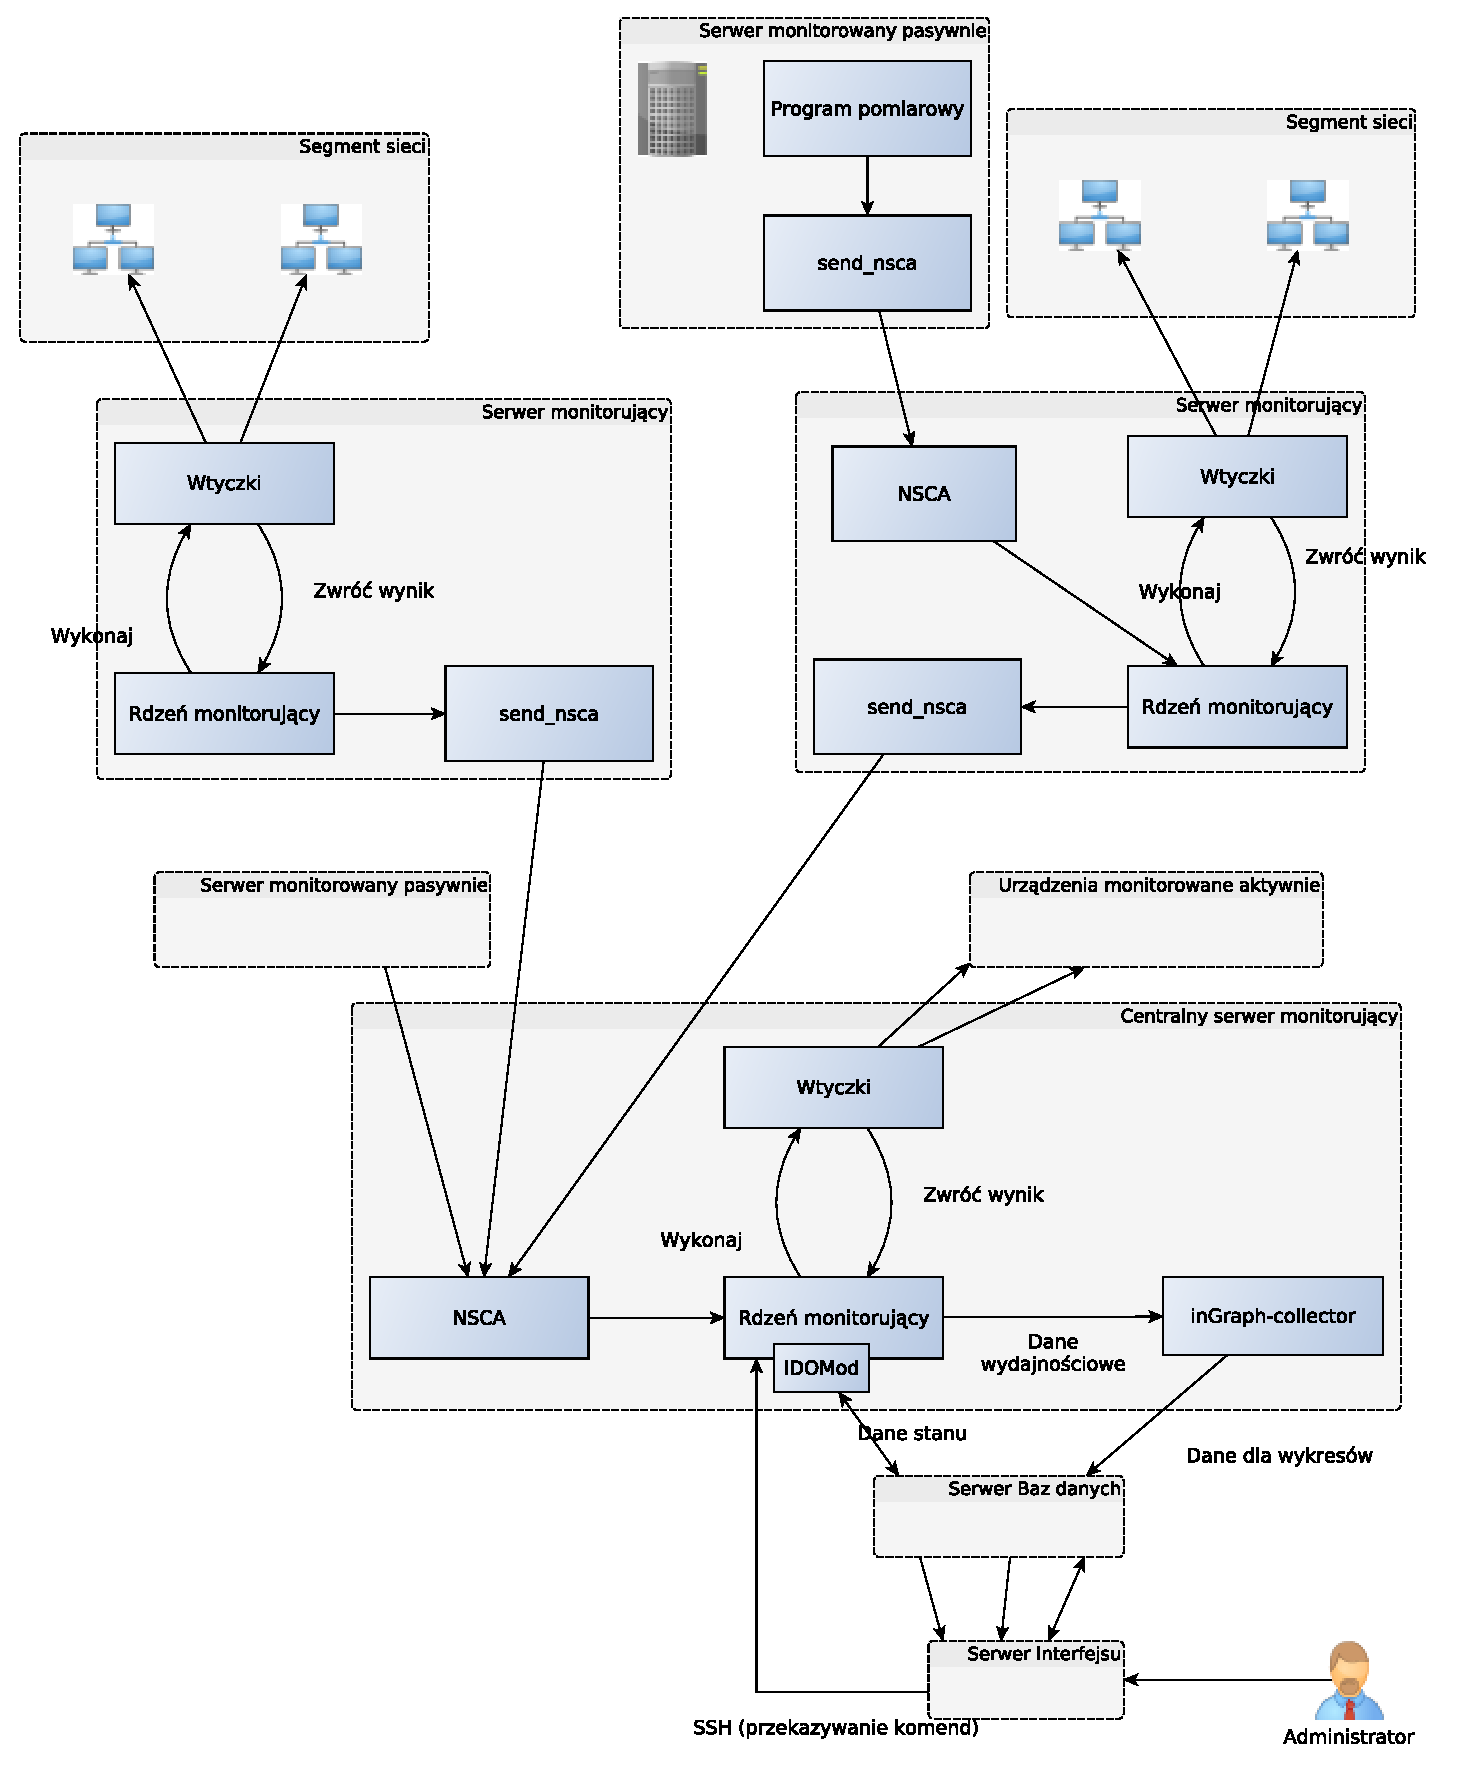
\includegraphics[width=1\textwidth]{img/icingaNSCA}
\end{figure}

Kolejnym z~możliwych scenariuszy współpracy wielu instancji rdzenia
monitorującego jest wykorzystanie wspólnej bazy danych. Rozwiązanie to
wymaga jedynie, aby wszystkie instancje rdzenia miały dostęp do jednej
bazy danych. Wszystkie instancje są w pełni niezależne i~każda z~nich
monitoruje w~dowolny sposób pewną grupę usług i~urządzeń. Wyniki
monitorowania są przetwarzane, przez każda instancję niezależnie, a~na
podstawie ich przetwarzania generowane są odpowiednie zdarzenia. Przy
użyciu komponentu IDOUtils wszystkie te dane są konsolidowane w
wspólnej bazie danych z~której korzysta interfejs icinga-web. Dzięki
wykorzystaniu nowego interfejsu możliwe jest równoczesna prezentacja
wyników monitorowania pochodzących od wielu instancji, przy użyciu
jednego interfejsu. Logiczny schemat tej konfiguracji przedstawiono na
\ref{fig:rozpFull}.

\begin{figure}[ht]
\centering
  \caption{Schemat konfiguracji rozproszonej ze~wspólną bazą danych.}
  \label{fig:rozpFull}
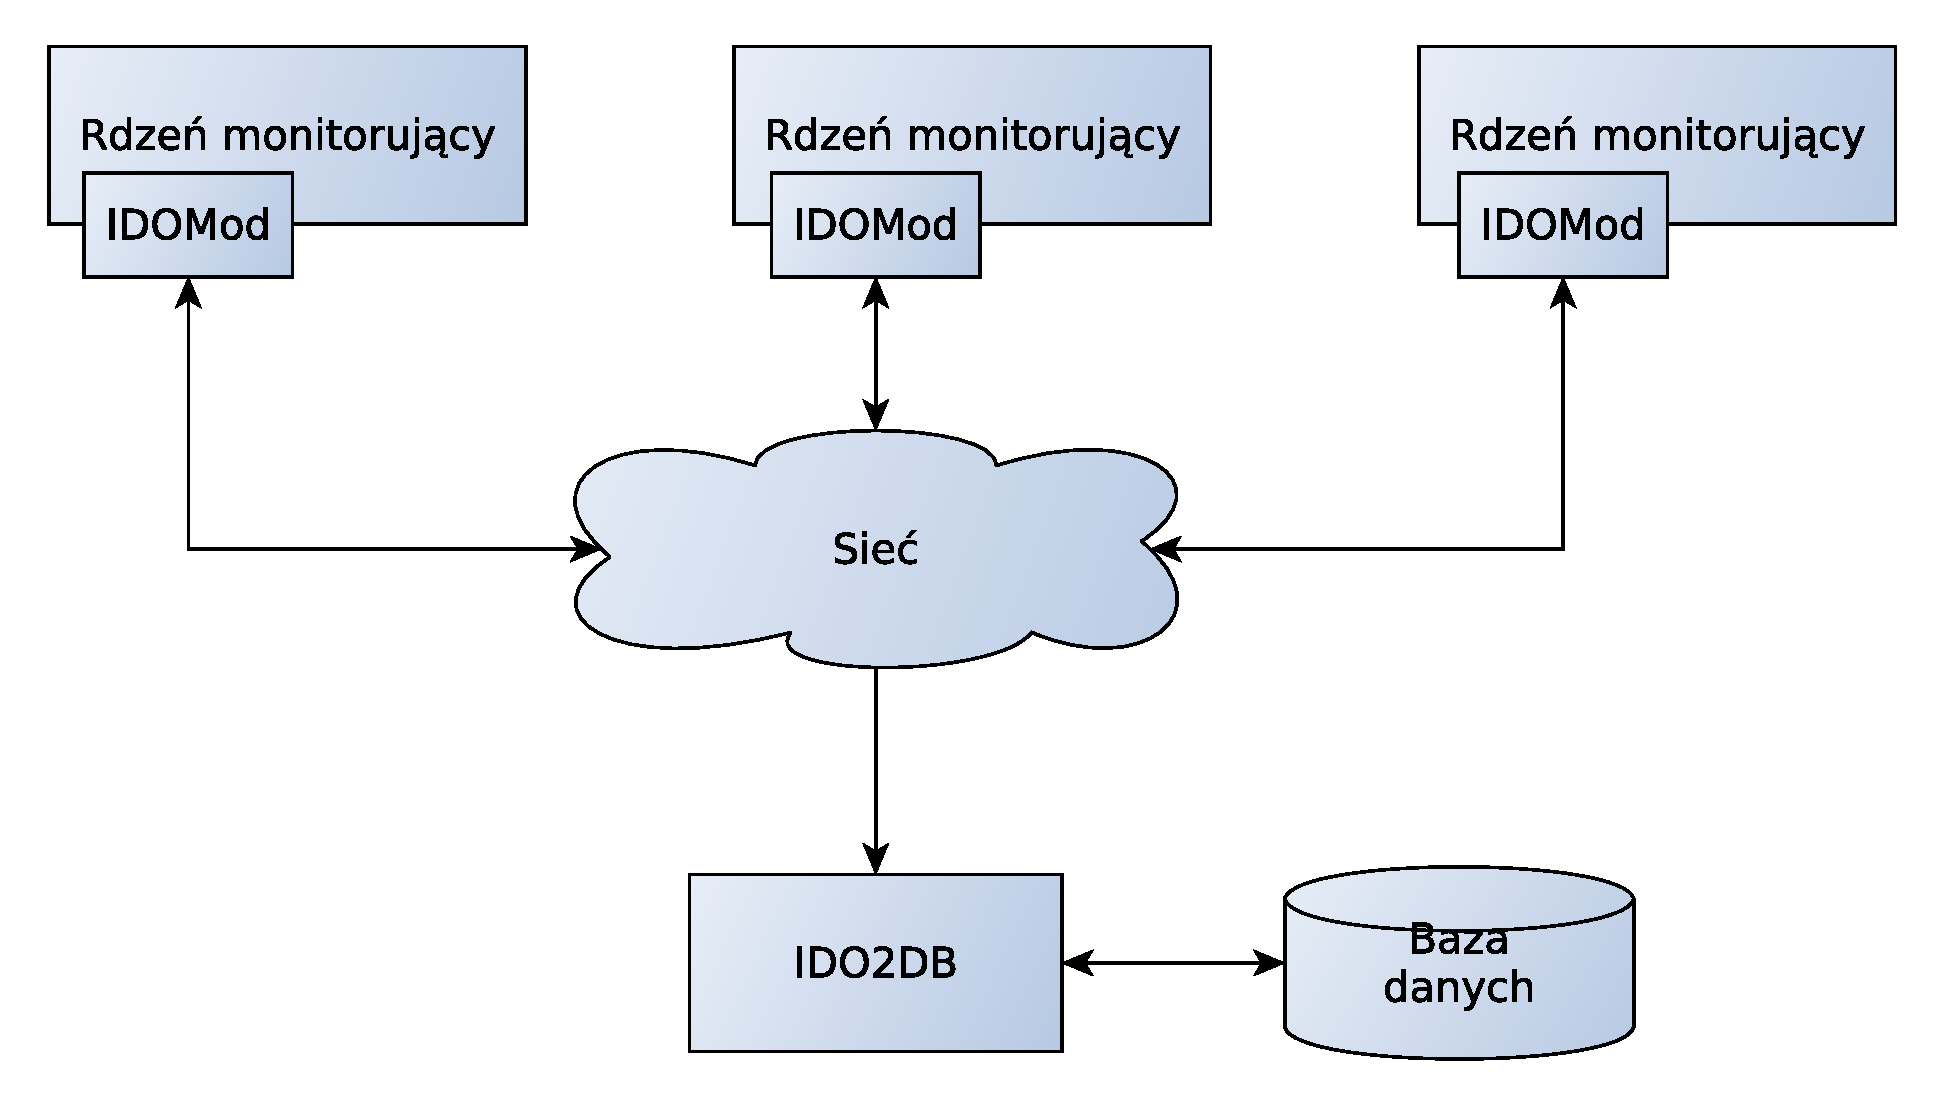
\includegraphics[width=0.8\textwidth]{img/icingaFull}
\end{figure}

Oba rozwiązania posiadają zarówno zalety jak i~wady. Rozwiązanie
z~użyciem dodatku NSCA zapewnia spójne przetwarzanie danych przez
jedna instancje i~łatwość konfiguracji dodatków wykorzystujących dane
eksportowane przez jądro w~postaci danych wydajnościowych. Niestety
rozwiązanie to generuje znaczące obciążenie instancji centralnej, gdyż
musi ona przetwarzać wszystkie wyniki sprawdzeń. Ponadto należy
przypomnieć, że model bezpieczeństwa dodatku NSCA posiada poważne
wady. Rozwiązanie oparte o~wspólną bazę danych posiada rozproszony
mechanizm przetwarzania sprawdzeń jak i~zdarzeń dzięki czemu nie
występuje w~nim nadmierne obciążenie jednej z~instancji. Ponadto
awaria, dowolnej z~instancji nie powoduje nigdy braku możliwości
monitorowania całej sieci lecz jedynie jej fragmentu. Niestety
w~rozwiązaniu tym konieczna jest bardziej zaawansowana konfiguracja
dodatków korzystających z~danych wydajnościowych. Wybór konfiguracji
zależy zatem silnie od infrastruktury w jakiej ma być ona zastosowana,
a także od pozostałych elementów systemu, jakie będą wykorzystane.


\section[Problemy][Problemy z monitorowaniem klienta mobilnego]{Problemy z monitorowaniem klienta mobilnego}

System Icinga nie posiada żadnego mechanizmu wsparcia dla klientów
mobilnych. Istnieje wiele konfiguracji rozproszonych, a~część z nich
może być zaadoptowana do monitorowania klienta mobilnego. Należy
pamiętać, iż element systemu obecny na urządzeniu mobilnym musi
oszczędzać zarówno pamięć jak i~czas procesora. Schemat logiczny
konfiguracji ze wspólną bazą danych dla klientów mobilnych został
przedstawiony na \ref{fig:mobilnyWspBaza}. Konfiguracja ta jest
niestety nieakceptowalna ze względu na konieczność przetwarzania
wszystkich informacji na urządzeniu mobilnym, co w~znaczący sposób
zwiększyłoby obciążenie klienta mobilnego.  W związku z~powyższym
zdecydowano się rozważyć konfigurację rozproszoną z~użyciem
NSCA. Wymaga ona dostarczenia elementu systemu, który będzie znajdował
się na urządzeniu mobilnym i monitorował je, a~następnie przekazywał,
gdy będzie to możliwe dane do instancji nadrzędnej, która będzie
prowadziła analizę otrzymanych danych. Schemat tej konfiguracji został
przedstawiony na \ref{fig:mobilnyInstancja}.

\begin{figure}[ht]
  \centering
  \caption{Monitoring klienta mobilnego w~konfiguracji ze~wspólną bazą
    danych.}
  \label{fig:mobilnyWspBaza}
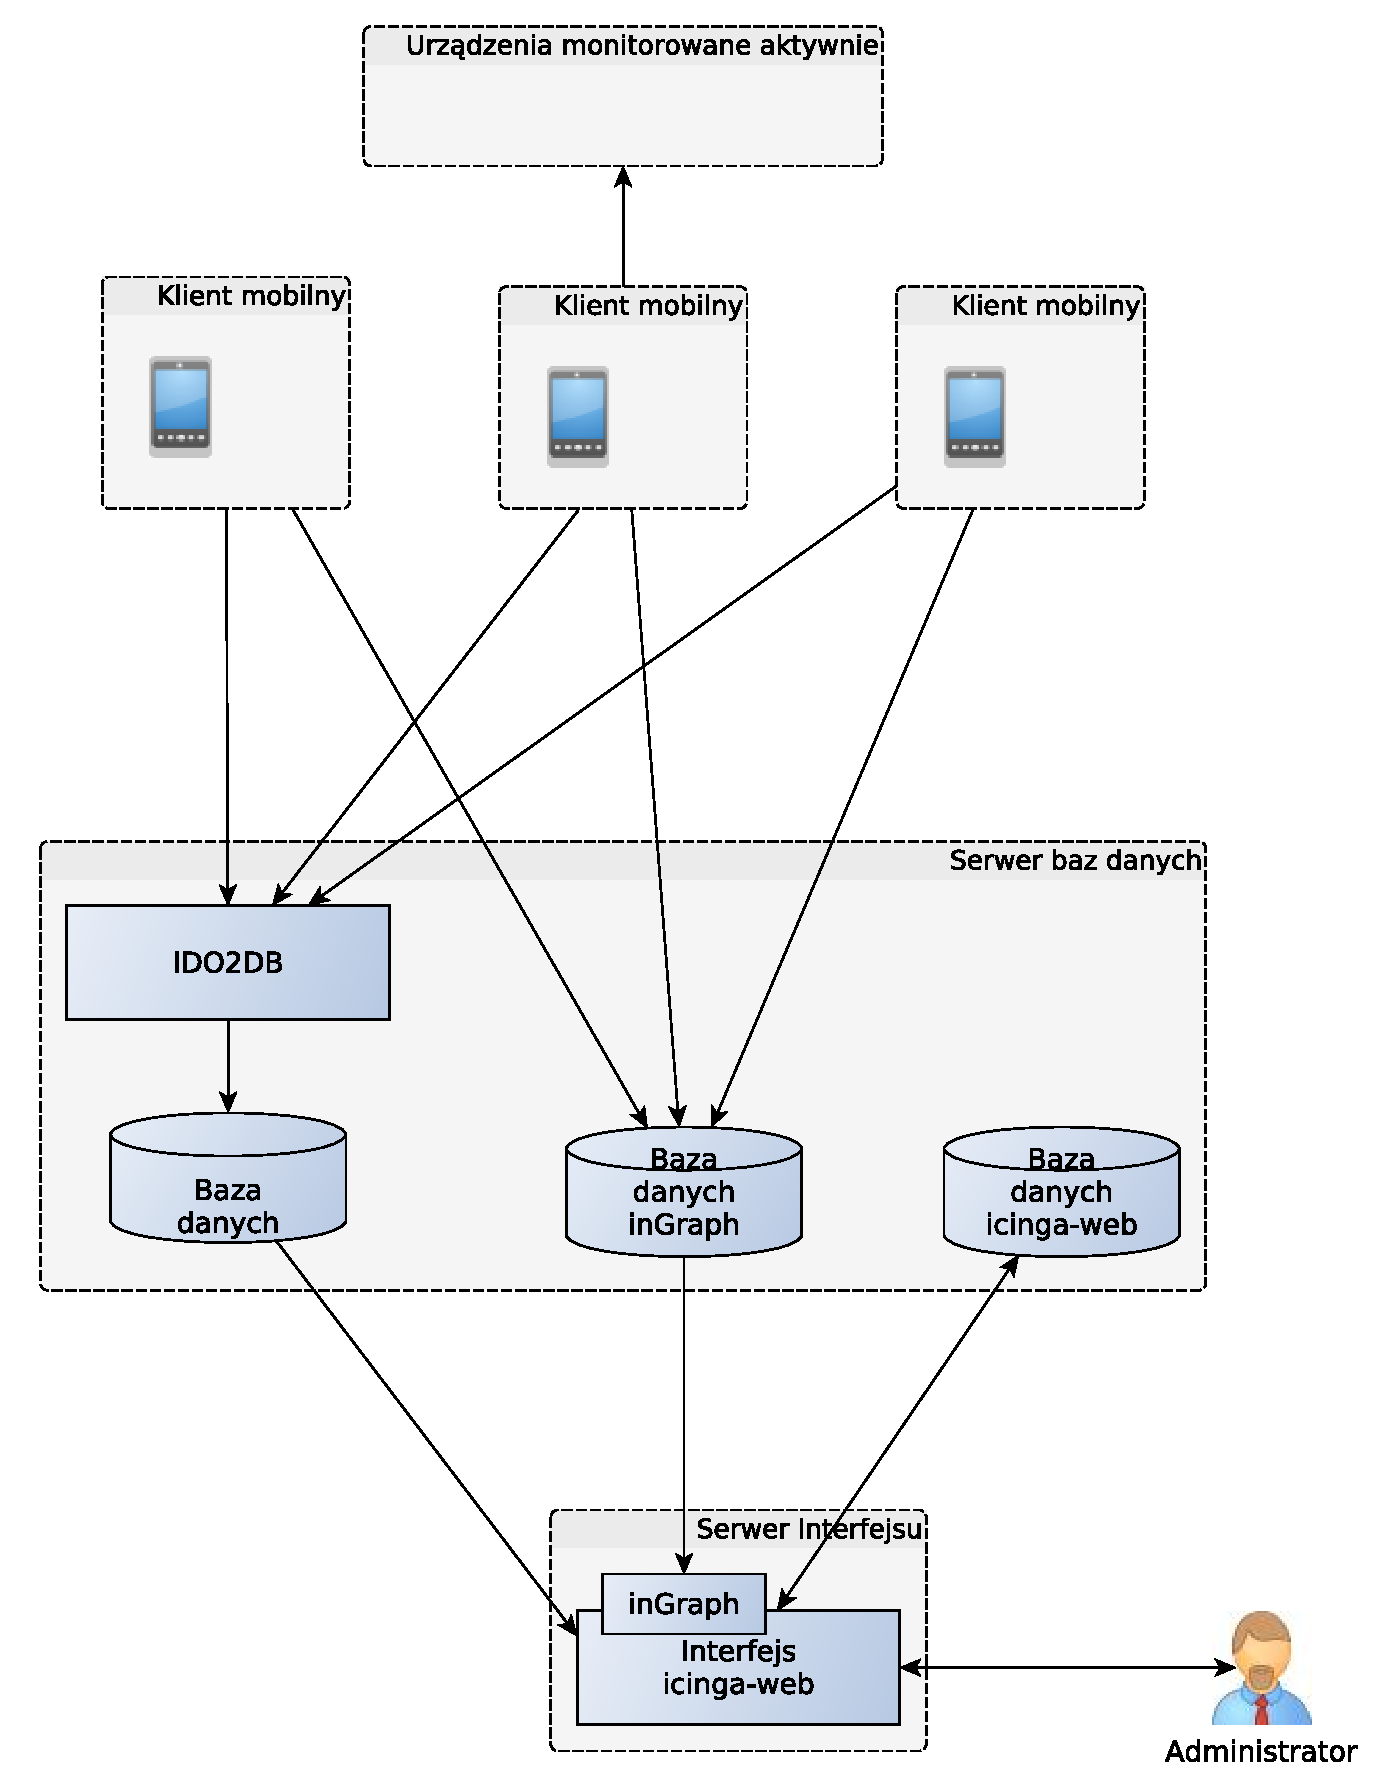
\includegraphics[width=0.75\textwidth]{img/mobilnyWspBaza}
\end{figure}

\begin{figure}[ht]
  \centering
  \caption{Monitoring klienta mobilnego w~konfiguracji z~instancją
    nadrzędną.}
  \label{fig:mobilnyInstancja}
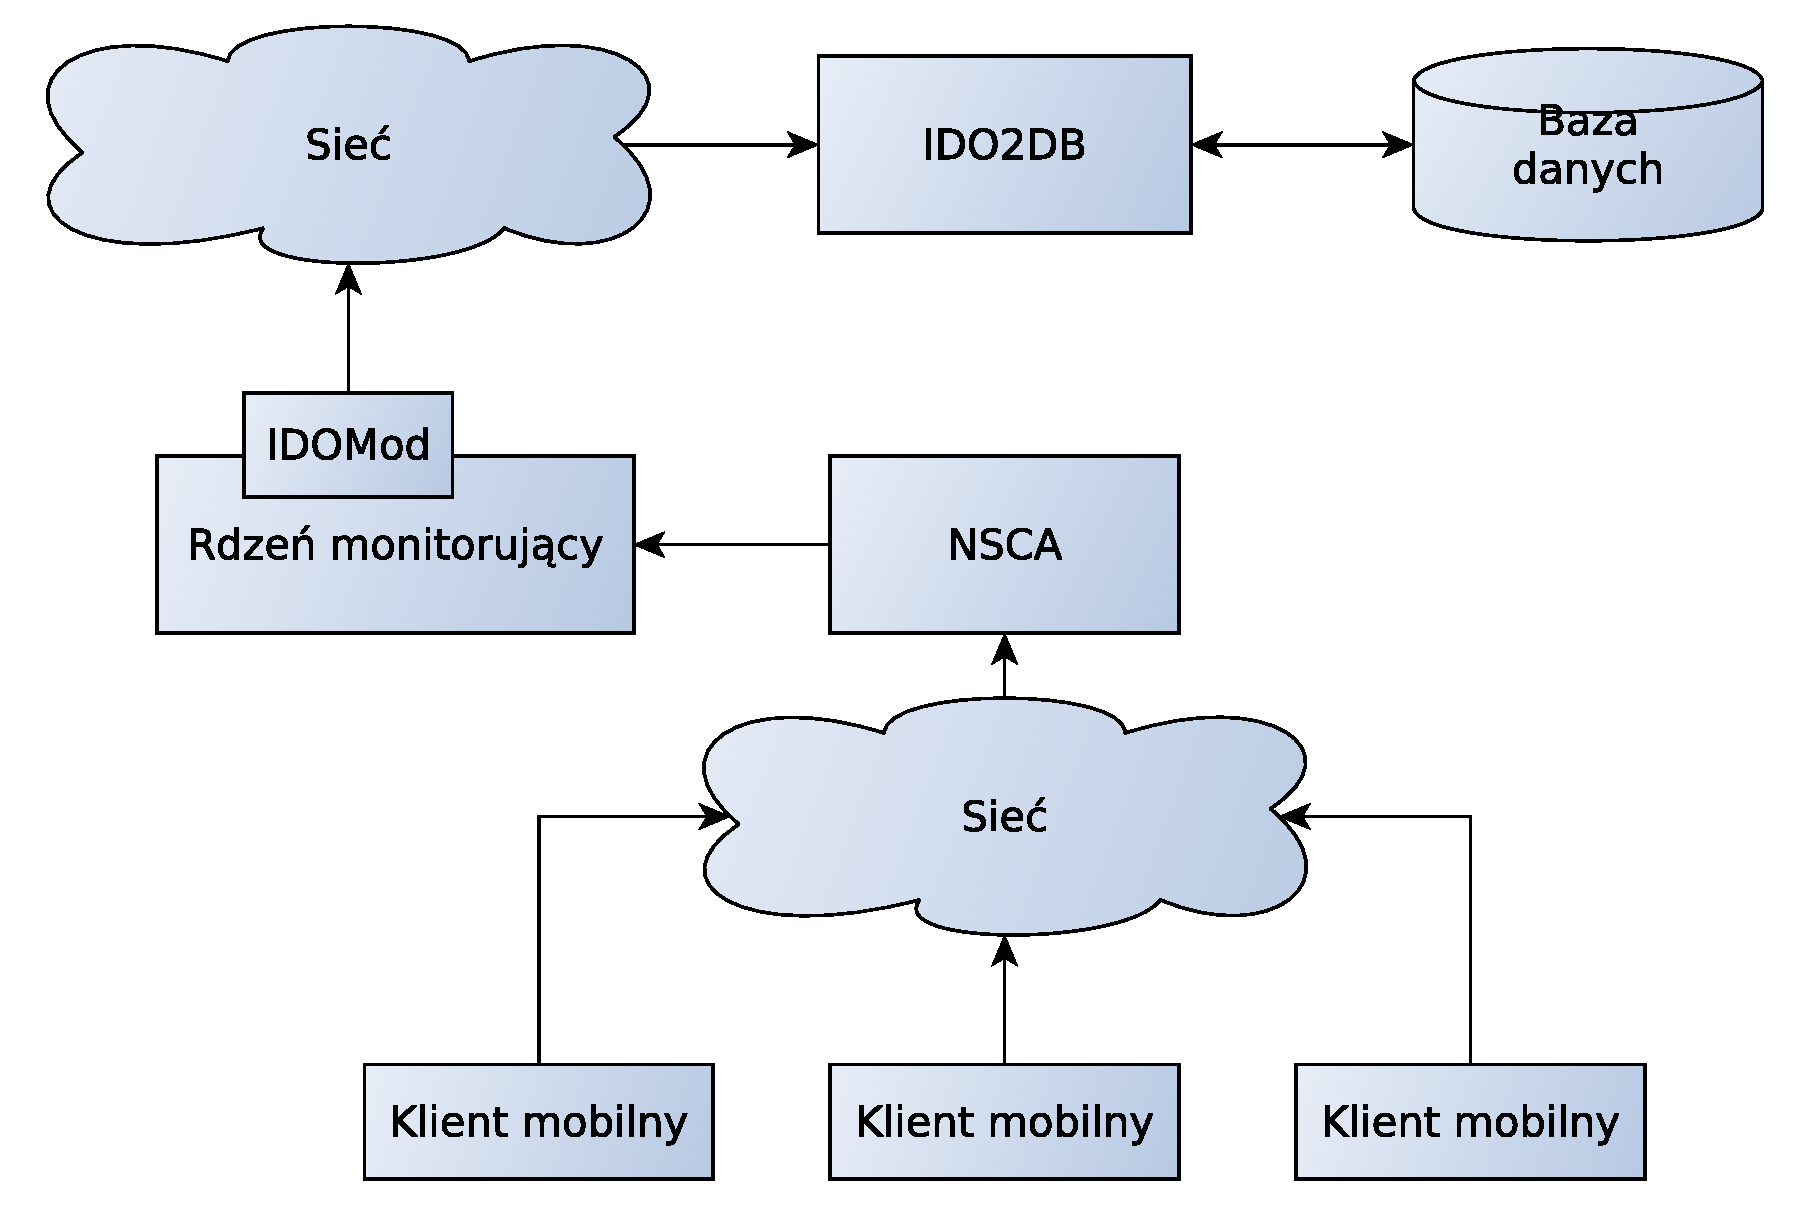
\includegraphics[width=0.80\textwidth]{img/mobilnyInstancja}
\end{figure}

Wykorzystanie do celu komunikacji pomiędzy klientem mobilnym,
a~instancja nadrzędną dodatku NSCA niesie za sobą wiele problemów.
Dodatek NSCA jest powszechnie używany do monitorowania serwerów
znajdujących się za zaporą lub w~wydzielonym segmencie sieci. Dodatek
ten może być stosowany, w~sieciach o~statycznym charakterze, gdzie
połączenia są stałe, a~łączność nie ulega częstym przerwaniom. Ponadto
należy być świadomym słabości modelu bezpieczeństwa stosowanego
w~protokole wymiany danych. Stosowanie dodatku NSCA poza zamkniętymi
sieciami firmowymi może okazać się niebezpieczne i~zawodne.

Zagadnienie monitorowania klienta mobilnego zostało szczegółowo
opisane w~\ref{chap:Wymagania}. Niestety dodatek NSCA nie spełnia
bardzo wielu z~przedstawionych wymagań przez co nie powinien być on
stosowany w~systemach tego typu. Głównymi problemami, które
dyskryminują ten w~zastosowaniu do monitorowania klienta mobilnego są:

\begin{description}
\item[Bezpieczeństwo] Mechanizmy bezpieczeństwa zawarte w~protokole
  wymiany danych posiadają poważne luki. Zastosowanie CRC32 do
  sprawdzania spójności danych niesie za sobą ryzyko ze względu na
  duże prawdopodobieństwo wystąpienia kolizji. Ponadto konieczność
  przechowywania na urządzeniu klucza symetrycznego, którego
  ujawnienie kompromituje cały system znacząco osłabia stosowane
  mechanizmy bezpieczeństwa.
\item[Nadpisywanie stempla czasu] Moduł odbierający dodaje do każdego
  wpisu dziennika aktualny stempel czasy. Powoduje to brak możliwości
  przesyłania, historycznych danych zgromadzonych w skutek utraty
  dostępu do sieci.
\item[Brak dodatkowych mechanizmów uwierzytelnienia klienta] Decyzja
  o~przydzieleniu klientowi dostępu czyli akceptacji przesłanych przez
  niego wpisów dziennika podejmowana jest na podstawie znajomości
  przez niego algorytmu szyfrowania oraz klucza.
\item[Brak kontroli otrzymywanych danych] Każdy klient, który zna
  klucz może przesyłać wpisy dotyczące dowolnego urządzenia i~dowolnej
  usługi. Brak jest mechanizmu, który pozwolił by na kontrolę tego,
  jaki klient ma prawo informować o~jakim urządzeniu czy też usłudze.
\item[Brak potwierdzenia dostarczenia danych] Klient wysyłający dane
  nie ma żadnej informacji o~tym, czy jego dane zostały zaakceptowane
  czy odrzucone. Oznacza to brak możliwości synchronizacji danych na
  kliencie mobilnym i~serwerze, gdyż nigdy nie mamy gwarancji, że
  wysłane przez klienta dane zostały przetworzone przez dodatek NSCA
  i~przekazane do rdzenia monitorującego.
\item[Brak implementacji dla systemów mobilnych] Moduł wysyłający jest
  aktualnie zaimplementowany jedynie na systemy Windows oraz
  Linux. Wiele współczesnych urządzeń mobilnych, które powinny być
  monitorowane funkcjonuje pod kontrolą systemu operacyjnego Android
  czy też Windows Phone.
\item[Przekazywanie danych tylko w~jedno miejsce] Dane odebrane przez
  moduł odbierający mogą być przekazane jedynie w~jedno miejsce. Przy
  bardziej złożonych systemach, konieczna jest możliwość przekazywania
  danych do kilku systemów oraz definiowania reguł, które dane gdzie
  powinny trafić.
\end{description}

Zastosowanie konfiguracji z~nadrzędną instancją rdzenia monitorującego
stanowi dobry szkielet dla systemu monitorowania klienta
mobilnego. Niestety dostępne na rynku narzędzie, to jest dodatek NSCA
nie są odpowiednio przystosowane do użycia ich w takim systemie. Wobec
braku dostępnych narzędzi na rynku konieczne jest zaprojektowanie oraz
zaimplementowanie nowego narzędzie, które spełni stawiane przed nim
wymagania.
